\noindent{\textbf{\underline{ニュースアンカーとして検出した発話の個数による評価}}}\par
k-meansによるニュースアンカーの発話の個数による発話検出精度を図\ref{fig:result_anchor_kmeans}、$Th_{time}$を変更してニュースアンカーの発話の個数による発話検出精度が最も高いF-measureを示した条件の結果を図\ref{fig:result_anchor_baseline} $\sim$ 図\ref{fig:result_anchor_prob3}に示す。その他の条件の結果は付録\ref{other_result}で記載する。また、図\ref{baseline_kmeans_fmeasure} $\sim$ 図\ref{prob3_fmeasure}に示された結果の中で、最も高いF-measureをとった$Th_{cos}$のときの各ニュース番組のニュースアンカーの発話検出精度とニュースアンカーとして検出したクラスタ数を表\ref{table:baseline_kmeans_eachnews} $\sim$ 表\ref{table:prob3_eachnews}に示す。

\begin{figure}[H]
  \centering
    \begin{tabular}{c}
 
%----- recall -----
 
      \begin{minipage}{0.40\hsize}
        \centering
          \subfigure[Recall]{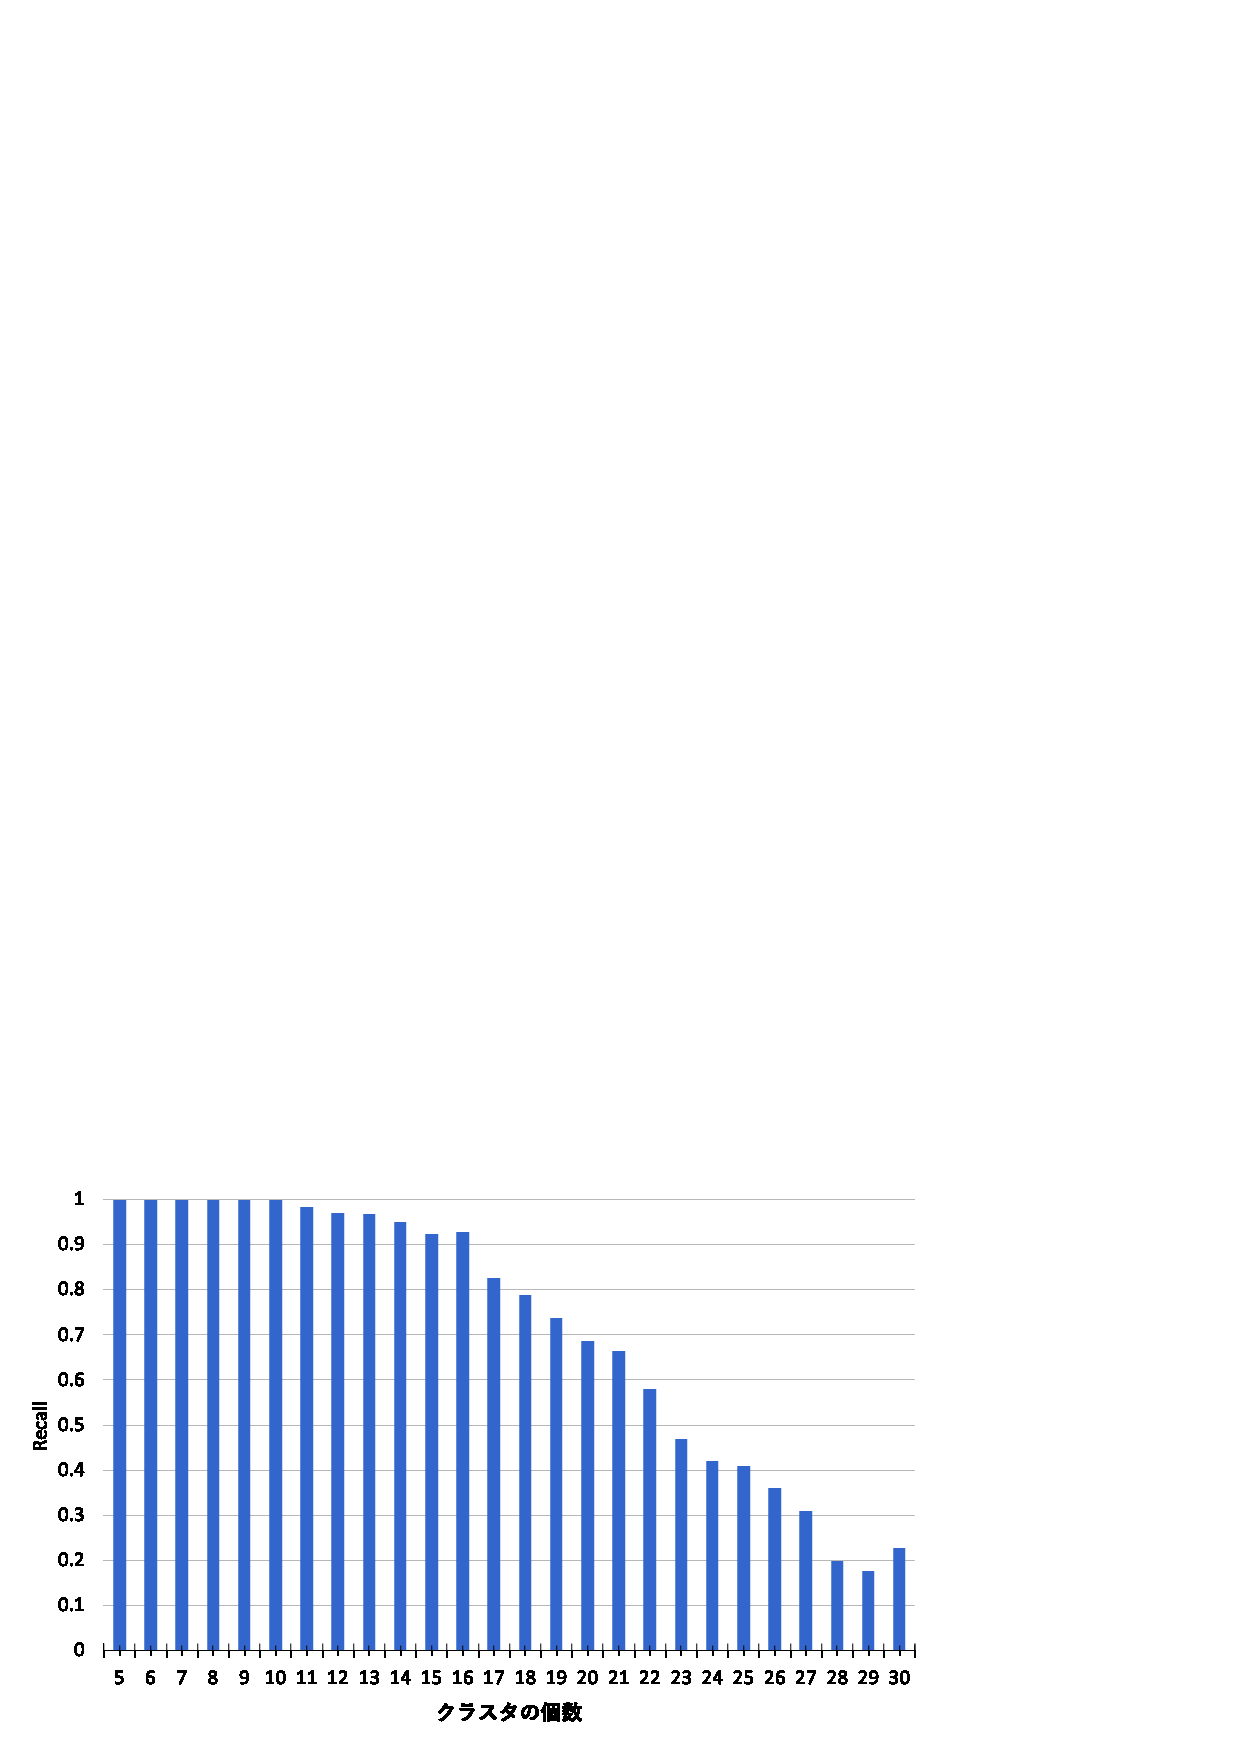
\includegraphics[keepaspectratio, scale=0.45]
                          {./figure/result_kmeans_r.eps}}
      \end{minipage}

      \begin{minipage}{0.06\hsize}
        \hspace{0.5mm}
      \end{minipage}
 
%----- precision -----
 
      \begin{minipage}{0.40\hsize}
        \centering
          \subfigure[Precision]{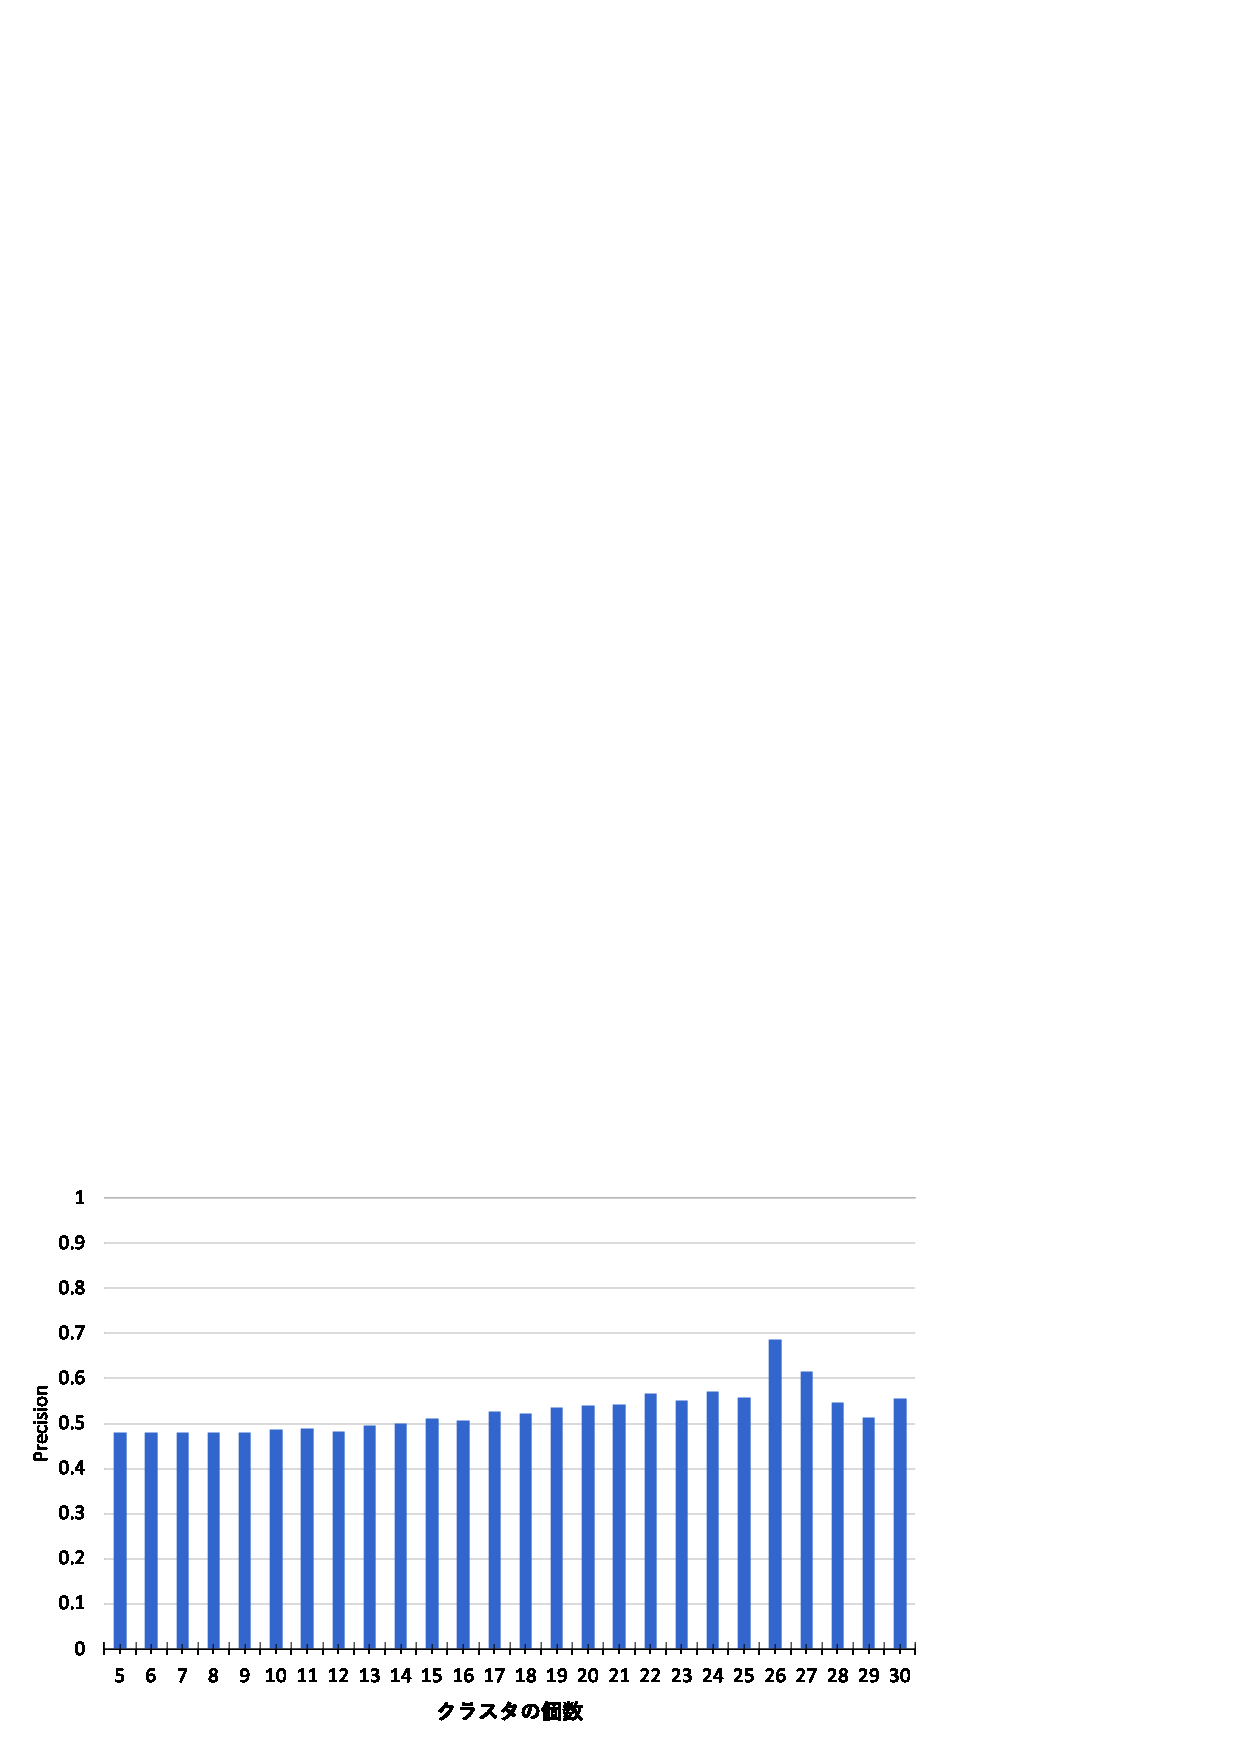
\includegraphics[keepaspectratio, scale=0.45]
                          {./figure/result_kmeans_p.eps}}
      \end{minipage} \\

      \begin{minipage}{0.06\hsize}
        \vspace{5mm}
      \end{minipage} \\
 
 
%----- fmeasure -----
 
      \begin{minipage}{0.40\hsize}
        \centering
          \subfigure[F-measure]{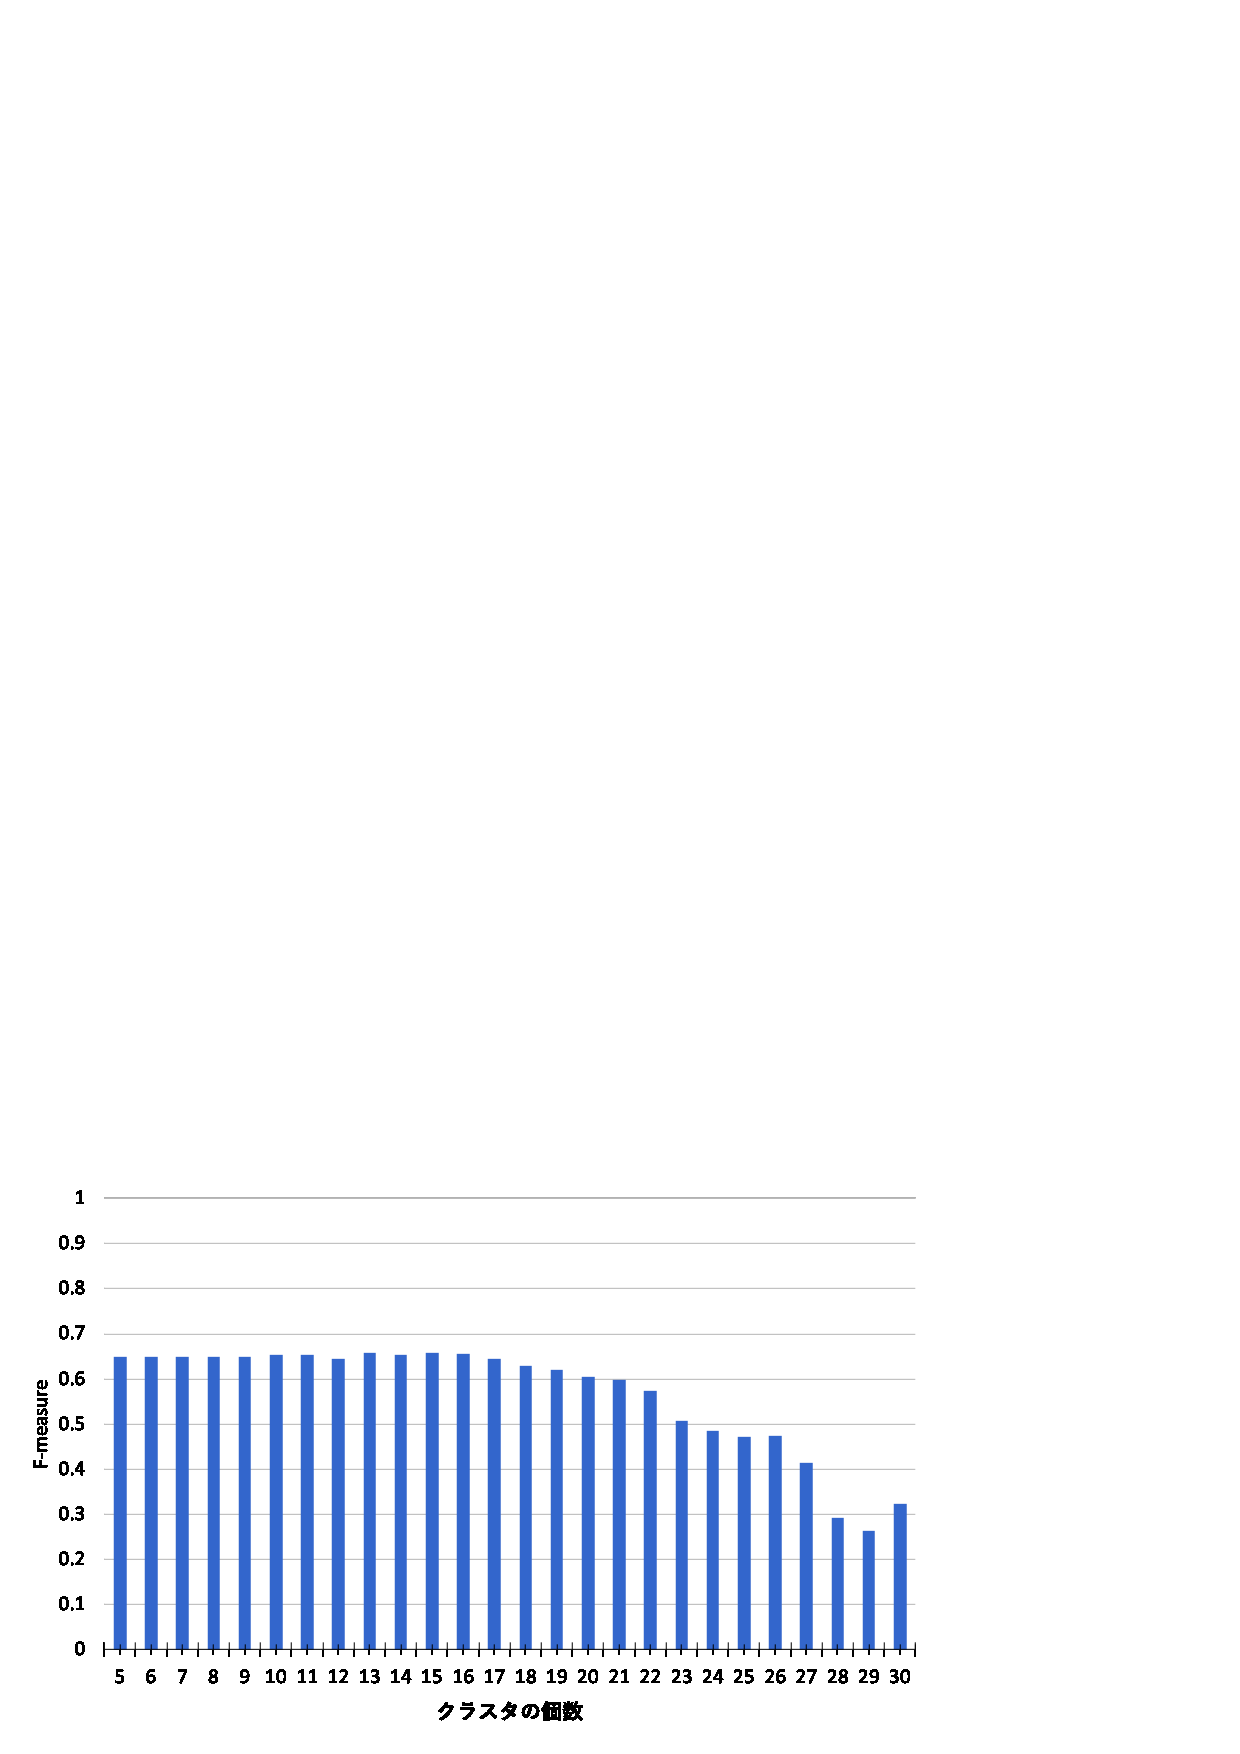
\includegraphics[keepaspectratio, scale=0.45]
                          {./figure/result_kmeans_f.eps} \label{baseline_kmeans_fmeasure}}
      \end{minipage}

      \begin{minipage}{0.06\hsize}
        \hspace{0.5mm}
      \end{minipage}


    \end{tabular}
\caption{Baseline1による発話区間検出精度 \label{fig:result_anchor_kmeans}}
\end{figure} 


\begin{table}[H]
  \begin{center}
    \caption{Baseline1による各ニュース番組音声のニュースアンカーの発話検出精度(クラスタの個数=13) \label{table:baseline_kmeans_eachnews}}
    \begin{tabular}{|c||c|c|c|c|} \hline
データID & Recall & Precision & F-meature & 作成したクラスタ数\\ \hline
ニュース1 & 0.970 & 0.578 & 0.724 & 6\\ \hline
ニュース2 & 1.000 & 0.334 & 0.501 & 12\\ \hline
ニュース3 & 1.000 & 0.485 & 0.653 & 14\\ \hline
ニュース4 & 0.955 & 0.545 & 0.694 & 12\\ \hline
ニュース5 & 0.981 & 0.623 & 0.762 & 12\\ \hline
計 & 0.961 & 0.495 & 0.645 & \\ \hline


    \end{tabular}
  \end{center}
\end{table}

\begin{figure}[H]
  \centering
    \begin{tabular}{c}
 
%----- recall -----
 
      \begin{minipage}{0.40\hsize}
        \centering
          \subfigure[Recall]{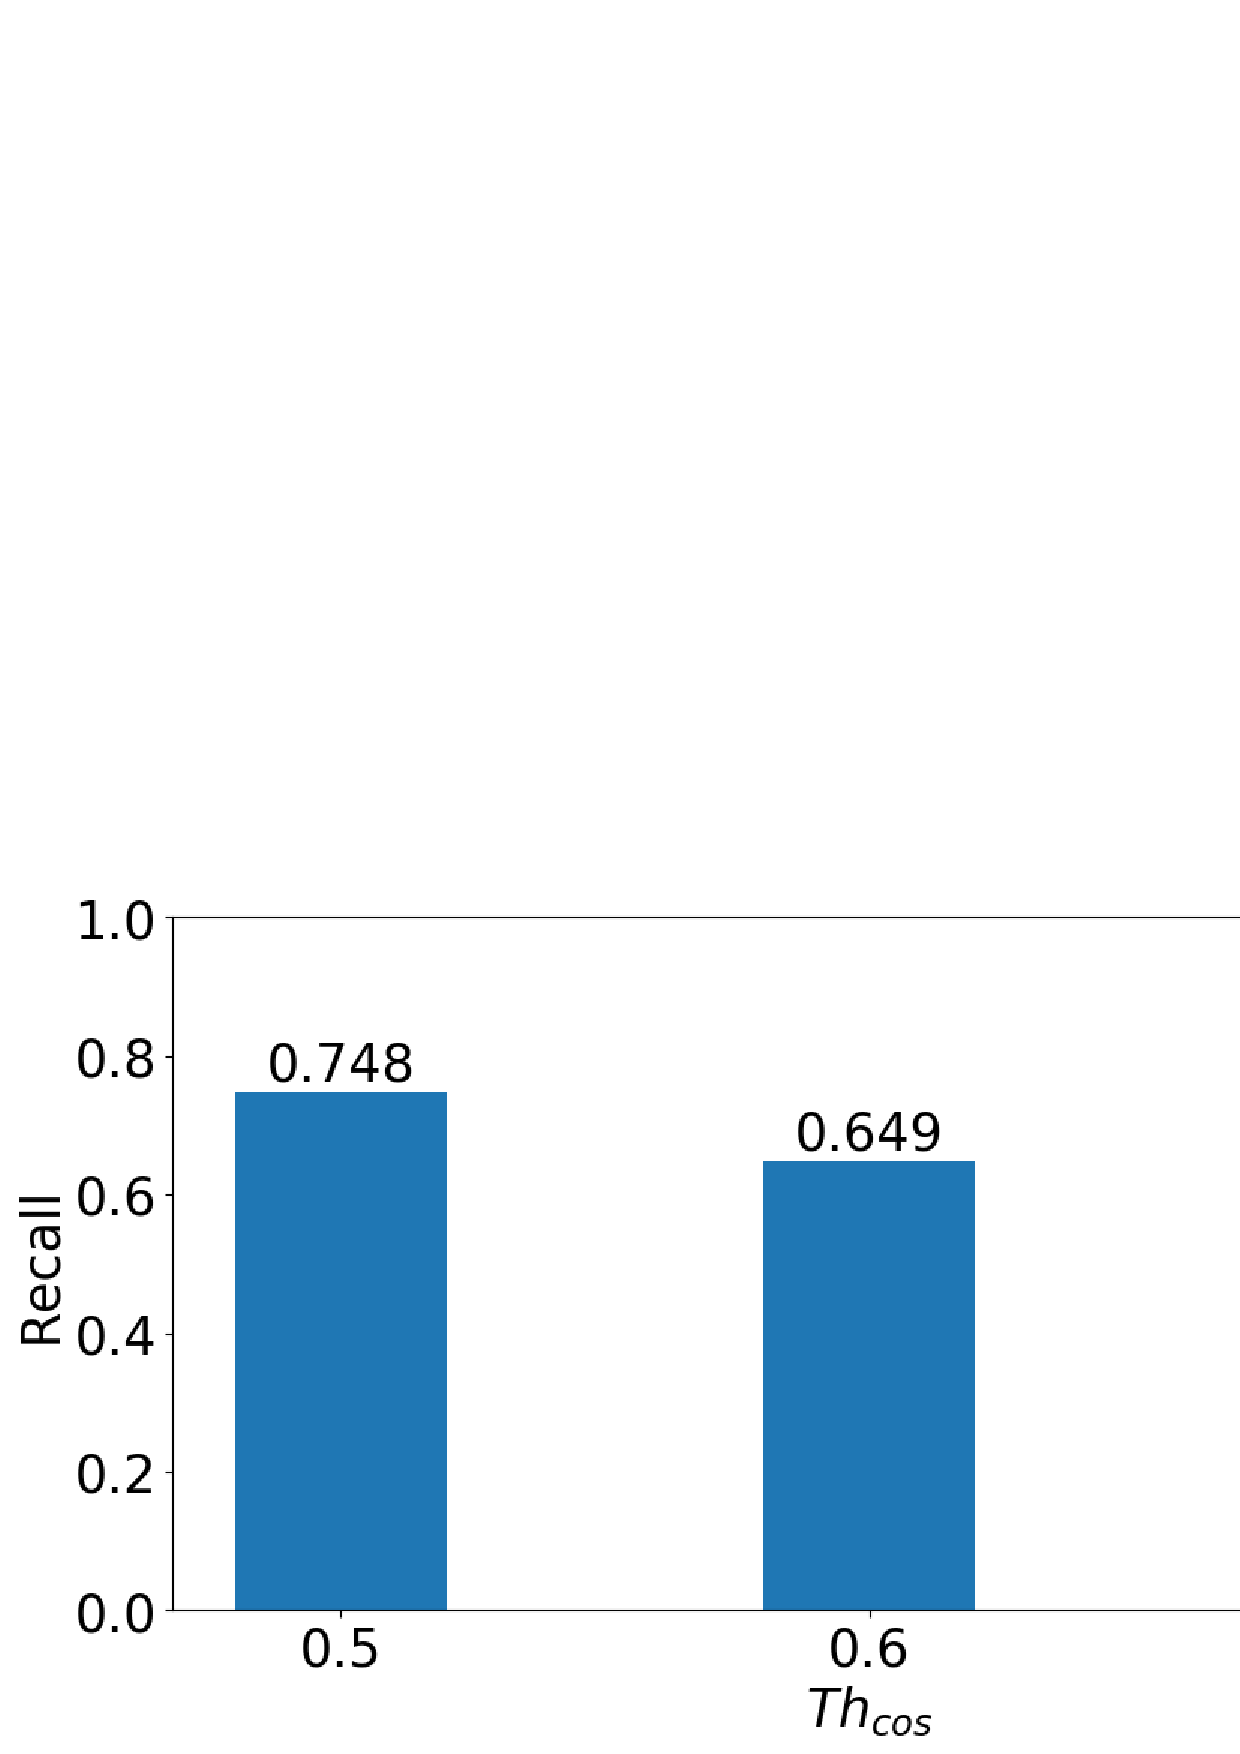
\includegraphics[keepaspectratio, scale=0.25]
                          {./figure/baseline_r.eps}}
      \end{minipage}

      \begin{minipage}{0.06\hsize}
        \hspace{0.5mm}
      \end{minipage}
 
%----- precision -----
 
      \begin{minipage}{0.40\hsize}
        \centering
          \subfigure[Precision]{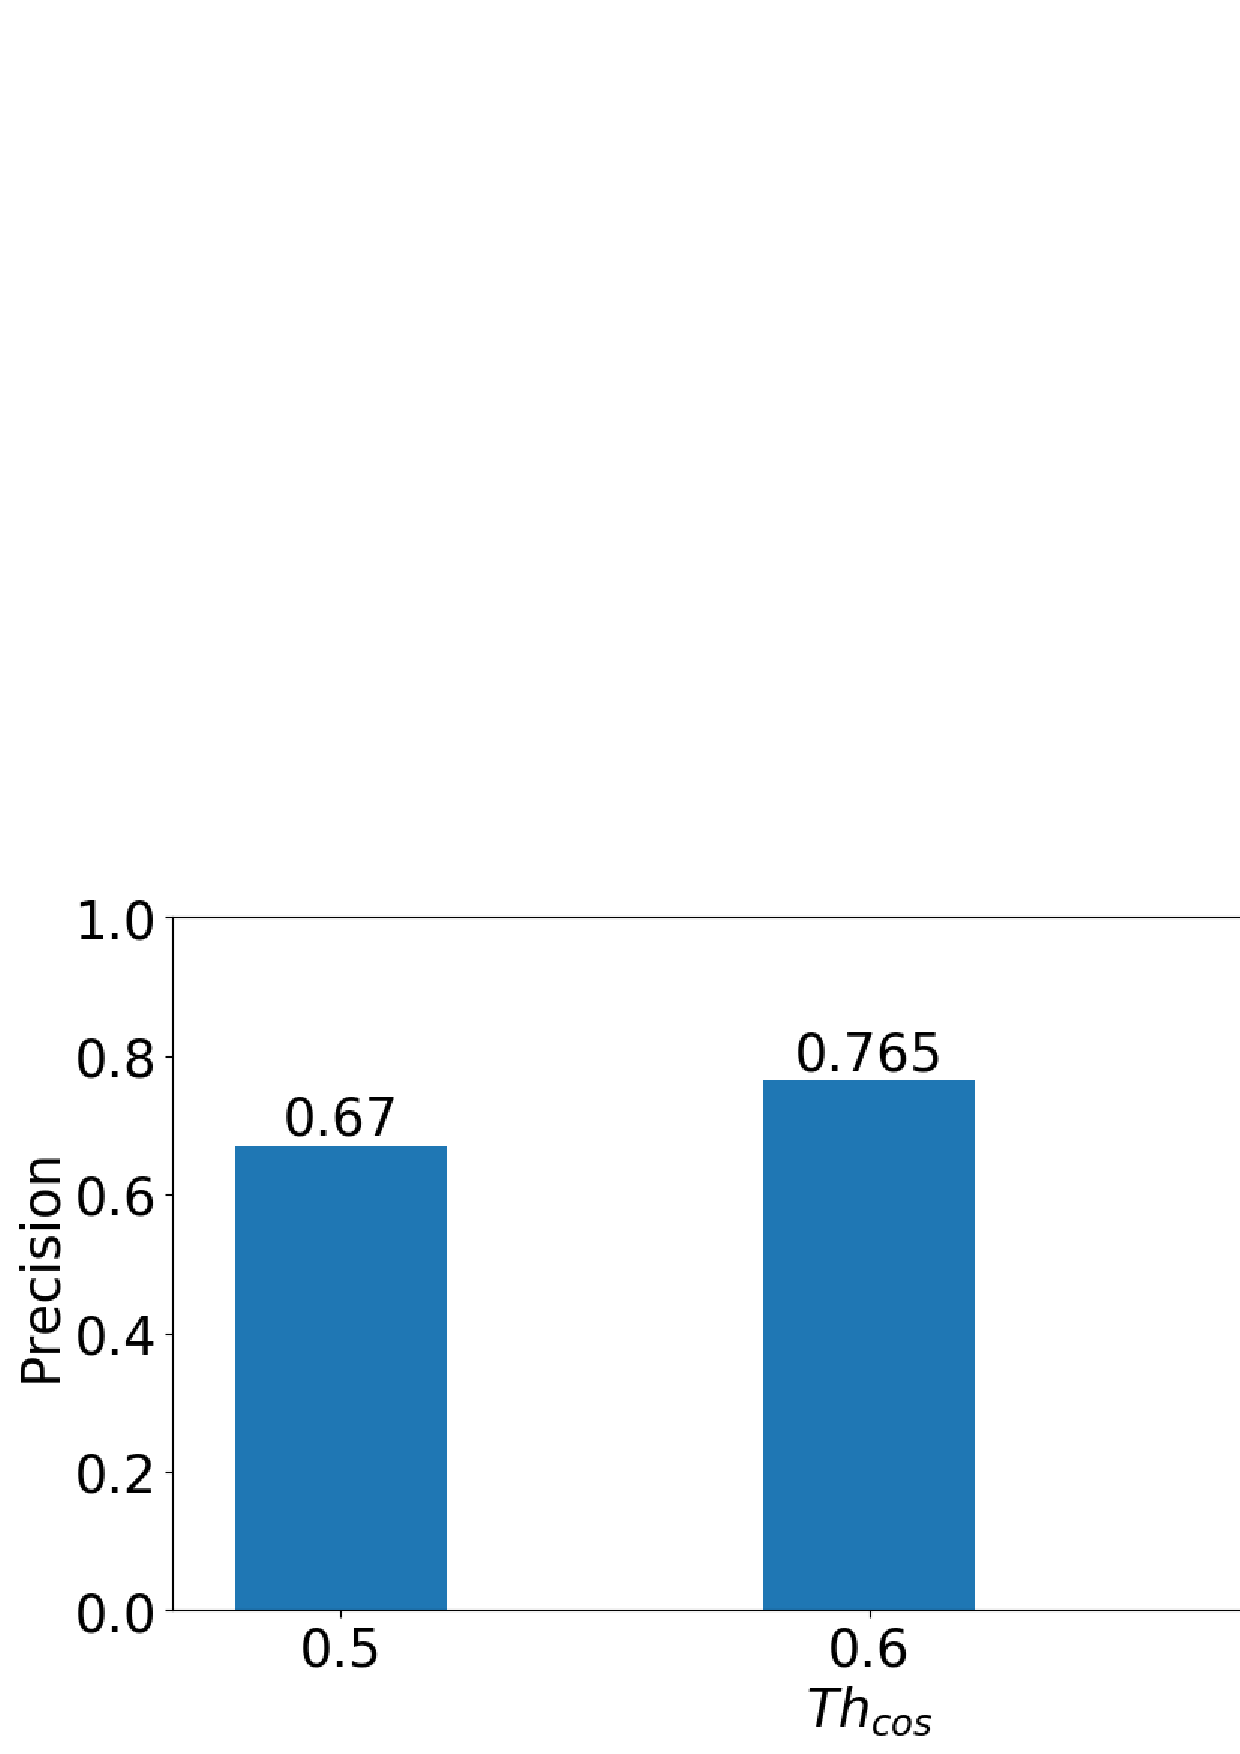
\includegraphics[keepaspectratio, scale=0.25]
                          {./figure/baseline_p.eps}}
      \end{minipage} \\

      \begin{minipage}{0.06\hsize}
        \vspace{5mm}
      \end{minipage} \\
 
 
%----- fmeasure -----
 
      \begin{minipage}{0.40\hsize}
        \centering
          \subfigure[F-measure]{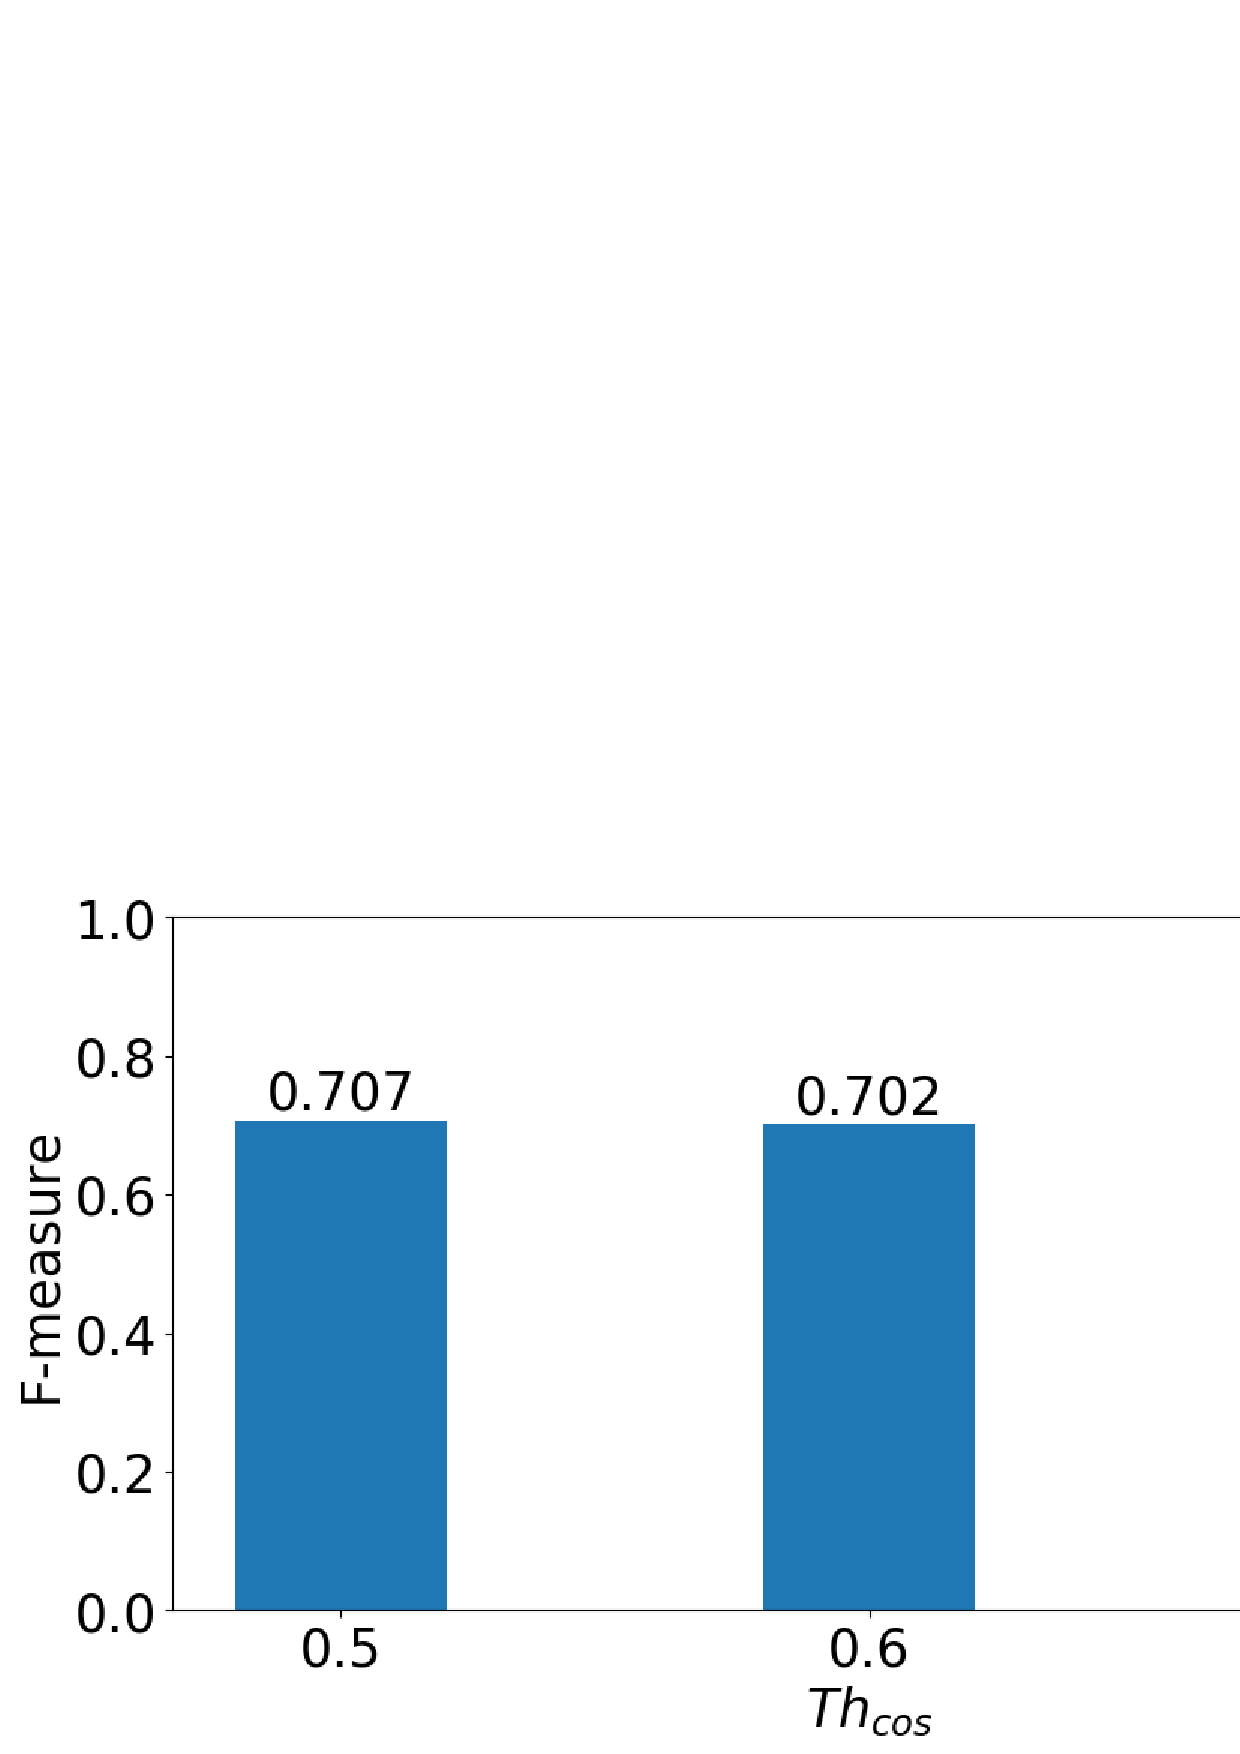
\includegraphics[keepaspectratio, scale=0.25]
                          {./figure/baseline_f.eps} }
      \end{minipage}

      \begin{minipage}{0.06\hsize}
        \hspace{0.5mm}
      \end{minipage}


    \end{tabular}
\caption{Baseline2による発話区間検出精度 \label{fig:result_anchor_baseline}}
\end{figure} 


\begin{table}[H]
  \begin{center}
    \caption{Baseline2による各ニュース番組音声のニュースアンカーの発話検出精度($Th_{cos}=0.5$) \label{table:baseline_eachnews}}
    \begin{tabular}{|c||c|c|c|c|} \hline
データID & Recall & Precision & F-meature & 作成したクラスタ数\\ \hline
ニュース1 & 0.970 & 0.623 & 0.758 & 1 \\ \hline
ニュース2 & 0.709 & 0.437 & 0.540 & 2 \\ \hline
ニュース3 & 0.736 & 0.719 & 0.727 & 2 \\ \hline
ニュース4 & 0.728 & 0.661 & 0.693 & 2 \\ \hline
ニュース5 & 0.683 & 0.947 & 0.793 & 2 \\ \hline
計 & 0.748 & 0.670 & 0.707 &  \\ \hline
    \end{tabular}
  \end{center}
\end{table}

%手法1の図
\begin{figure}[H]
  \centering
    \begin{tabular}{c}
 
%----- recall -----
 
      \begin{minipage}{0.40\hsize}
        \centering
          \subfigure[Recall]{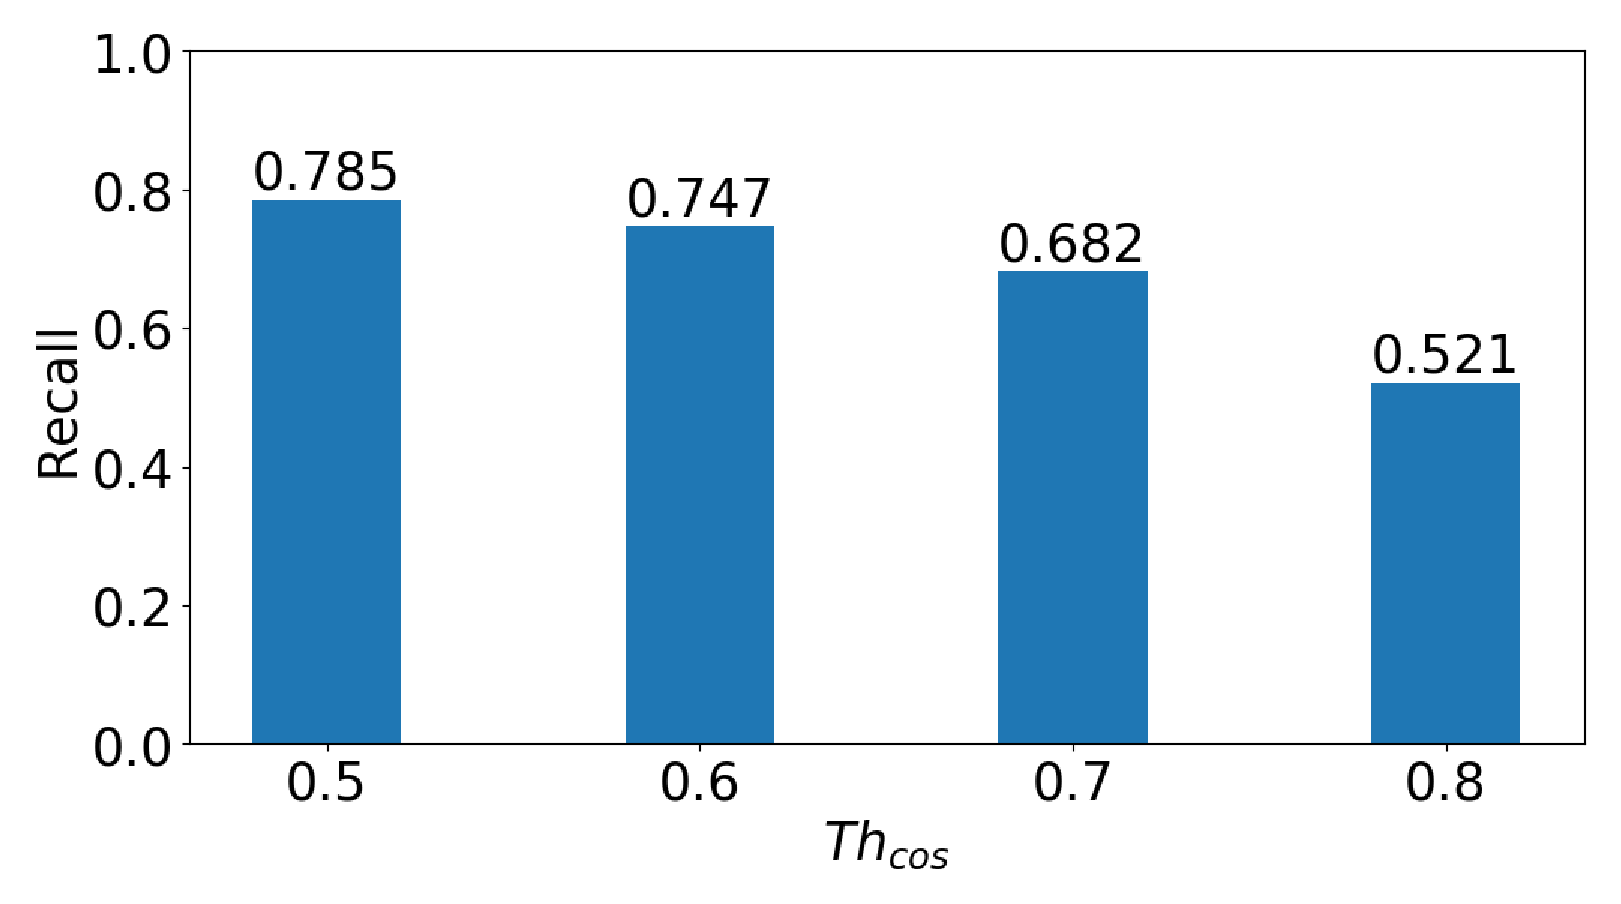
\includegraphics[keepaspectratio, scale=0.25]
                          {./figure/prob1_12_r.eps}}
      \end{minipage}

      \begin{minipage}{0.06\hsize}
        \hspace{0.5mm}
      \end{minipage}
 
%----- precision -----
 
      \begin{minipage}{0.40\hsize}
        \centering
          \subfigure[Precision]{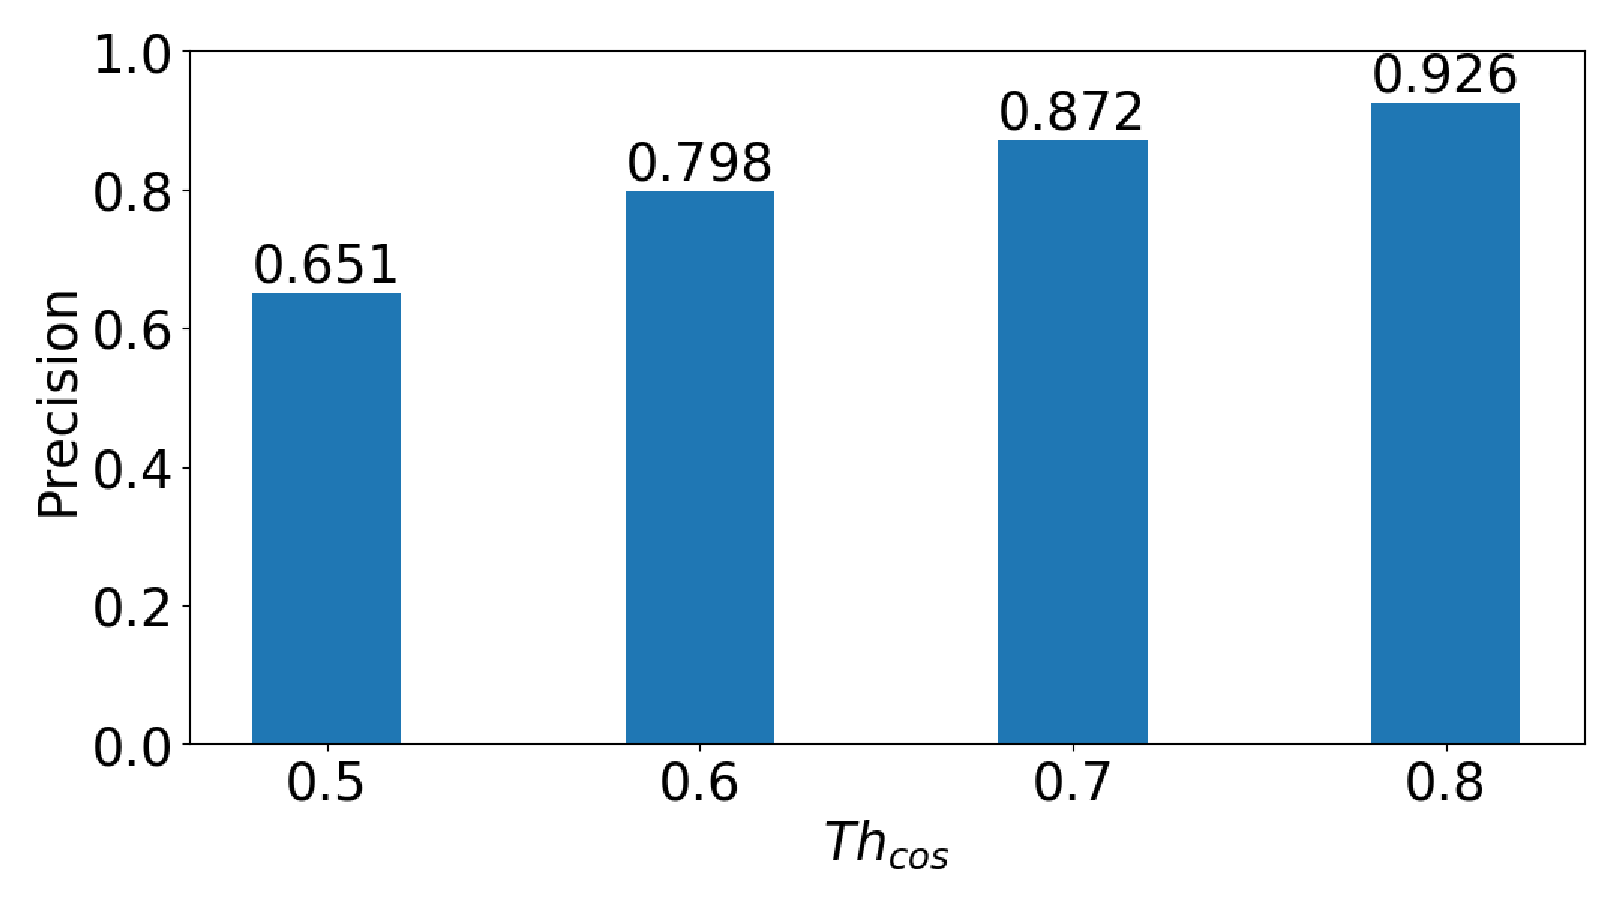
\includegraphics[keepaspectratio, scale=0.25]
                          {./figure/prob1_12_p.eps}}
      \end{minipage} \\

      \begin{minipage}{0.06\hsize}
        \vspace{5mm}
      \end{minipage} \\
 
 
%----- fmeasure -----
 
      \begin{minipage}{0.40\hsize}
        \centering
          \subfigure[F-measure]{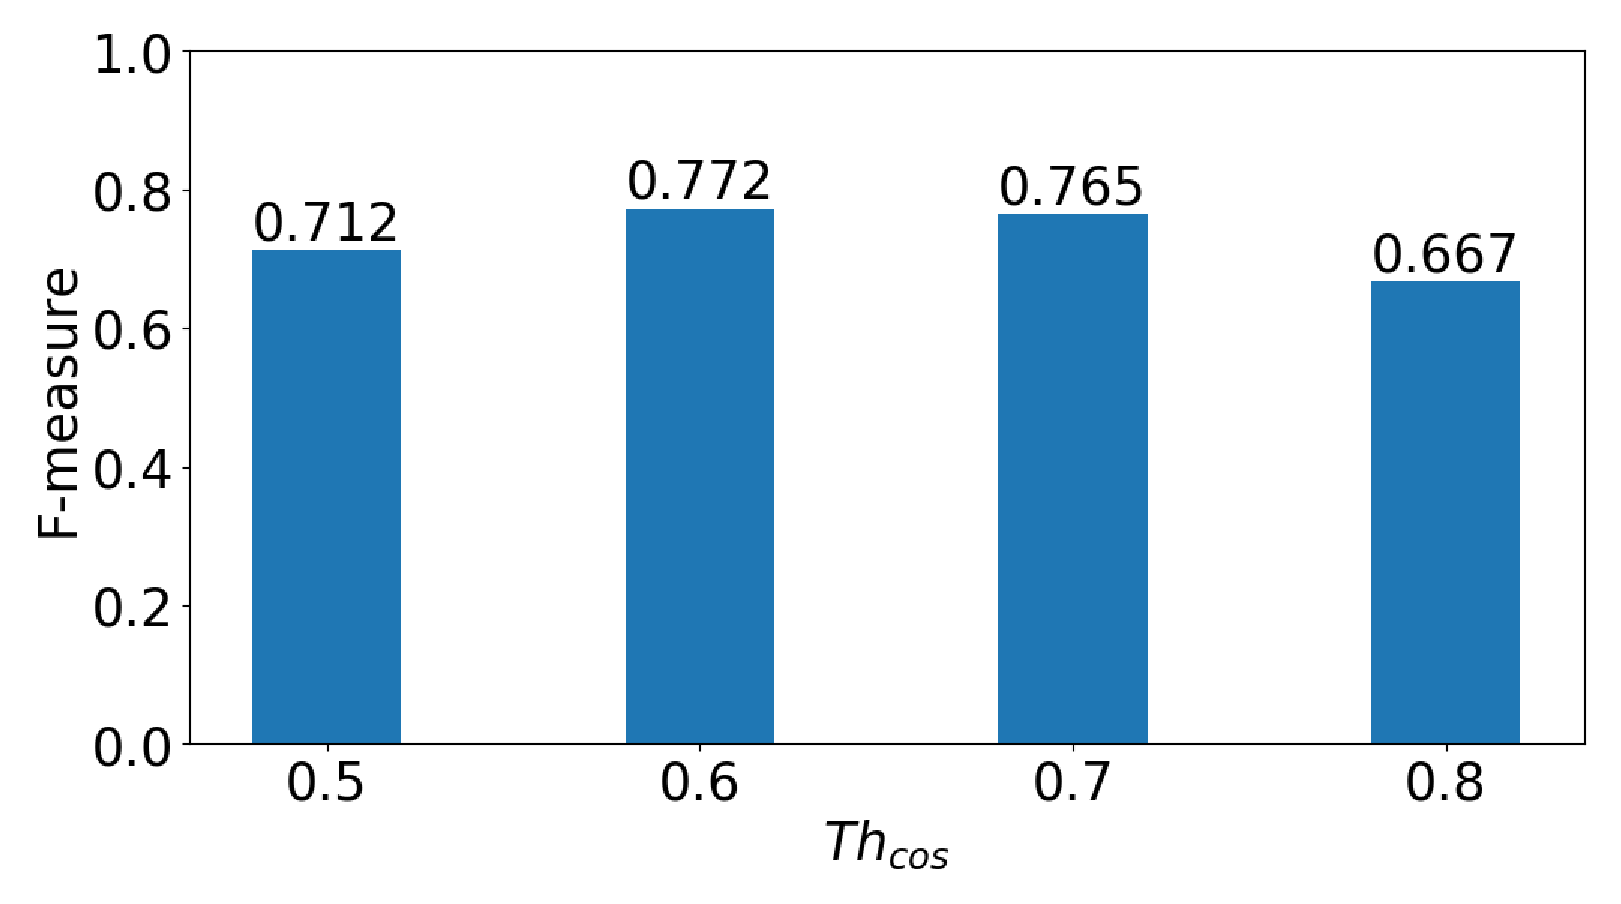
\includegraphics[keepaspectratio, scale=0.25]
                          {./figure/prob1_12_f.eps} \label{prob1_fmeasure}}
      \end{minipage}

      \begin{minipage}{0.06\hsize}
        \hspace{0.5mm}
      \end{minipage}
 

    
    \end{tabular}
\caption{手法1によるアンカーの発話区間検出精度 ($Th_{time}=1.2$) \label{fig:result_anchor_prob1}}
\end{figure} 

\begin{table}[H]
  \begin{center}
    \caption{手法1による各ニュース番組音声のニュースアンカーの発話検出精度($Th_{cos}=0.6,Th_{time}=1.2$) }
    \begin{tabular}{|c||c|c|c|c|} \hline
データID & Recall & Precision & F-meature & 作成したクラスタ数\\ \hline
ニュース1 & 0.964 & 0.707 & 0.815 & 1 \\ \hline
ニュース2 & 0.764 & 0.685 & 0.722 & 2 \\ \hline
ニュース3 & 0.729 & 0.860 & 0.789 & 2 \\ \hline
ニュース4 & 0.683 & 0.741 & 0.711 & 2 \\ \hline
ニュース5 & 0.695 & 0.978 & 0.813 & 2 \\ \hline
計 & 0.747 & 0.798 & 0.765 &  \\ \hline
    \end{tabular}
  \end{center}
\end{table}

%手法2の図
\begin{figure}[H]
  \centering
    \begin{tabular}{c}
 
%----- recall -----
 
      \begin{minipage}{0.40\hsize}
        \centering
          \subfigure[Recall]{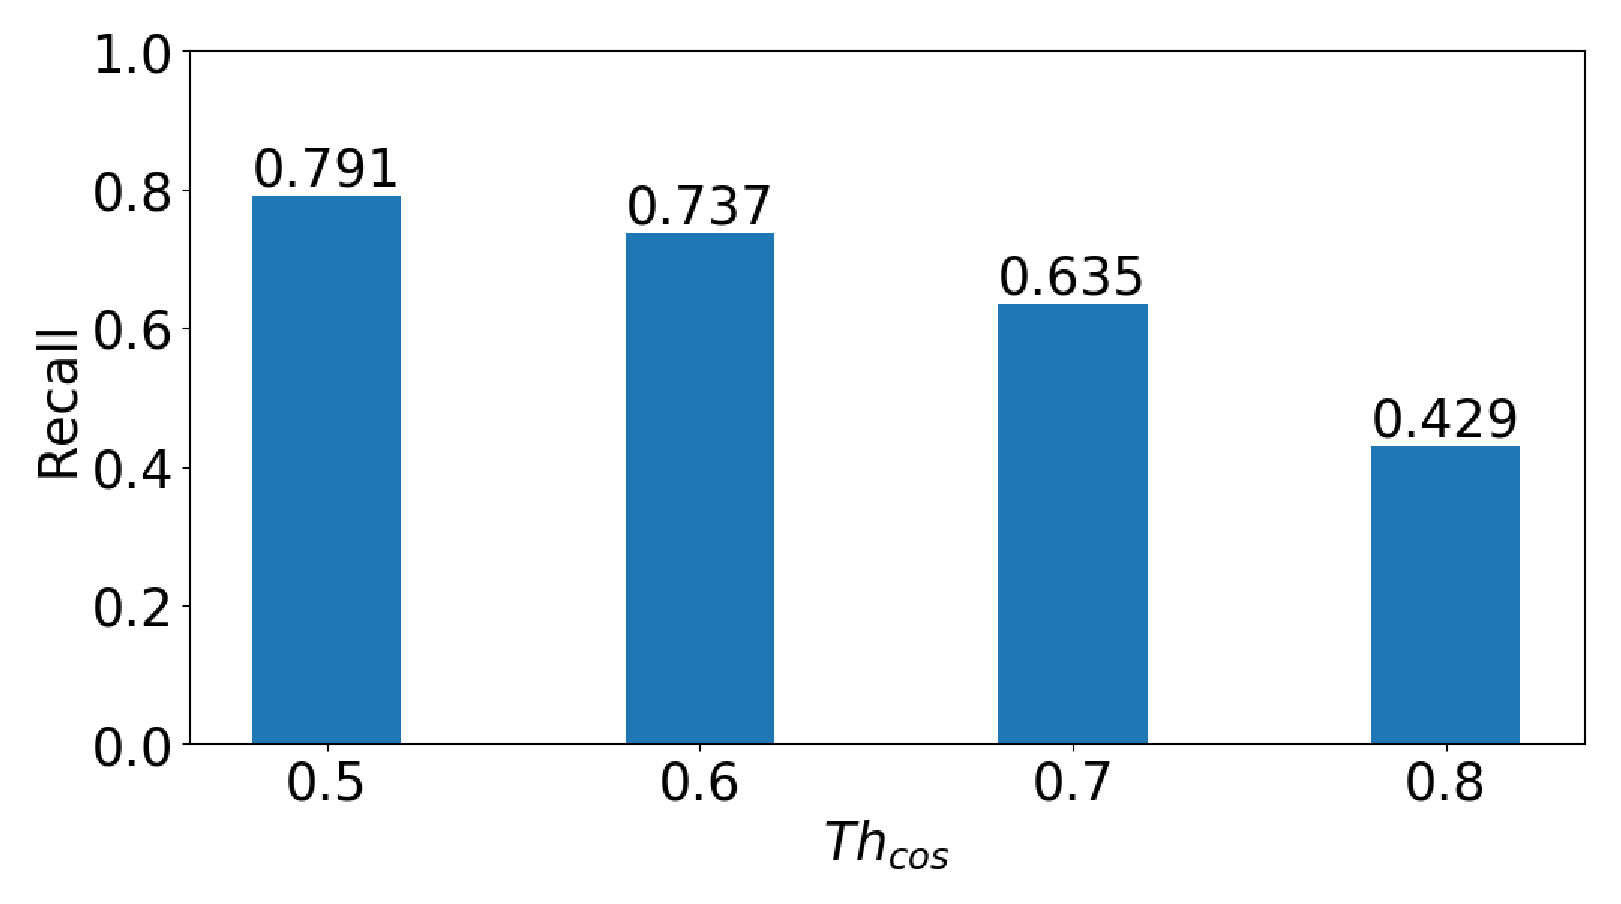
\includegraphics[keepaspectratio, scale=0.25]
                          {./figure/prob2_r.eps}}
      \end{minipage}

      \begin{minipage}{0.06\hsize}
        \hspace{0.5mm}
      \end{minipage}
 
%----- precision -----
 
      \begin{minipage}{0.40\hsize}
        \centering
          \subfigure[Precision]{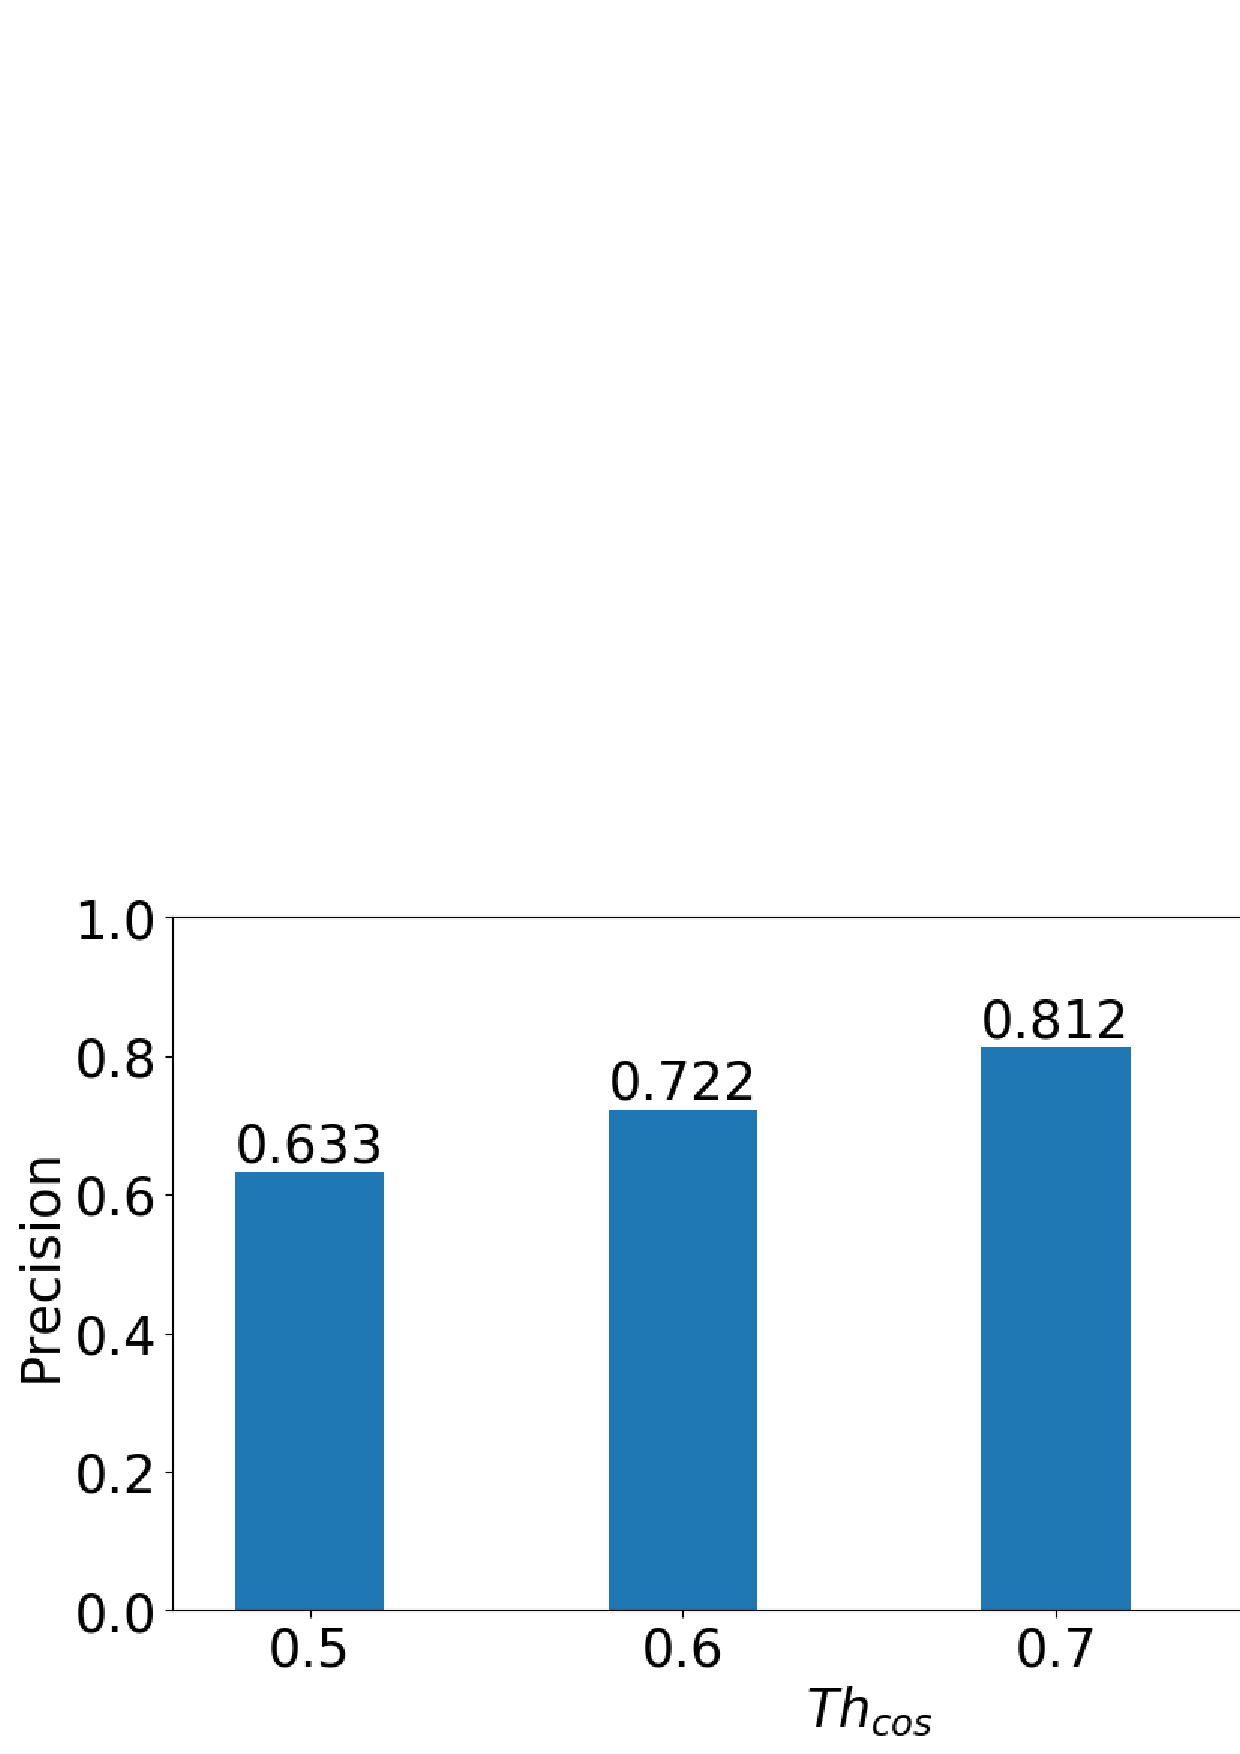
\includegraphics[keepaspectratio, scale=0.25]
                          {./figure/prob2_p.eps}}
      \end{minipage} \\

      \begin{minipage}{0.06\hsize}
        \vspace{5mm}
      \end{minipage} \\
 
 
%----- fmeasure -----
 
      \begin{minipage}{0.40\hsize}
        \centering
          \subfigure[F-measure]{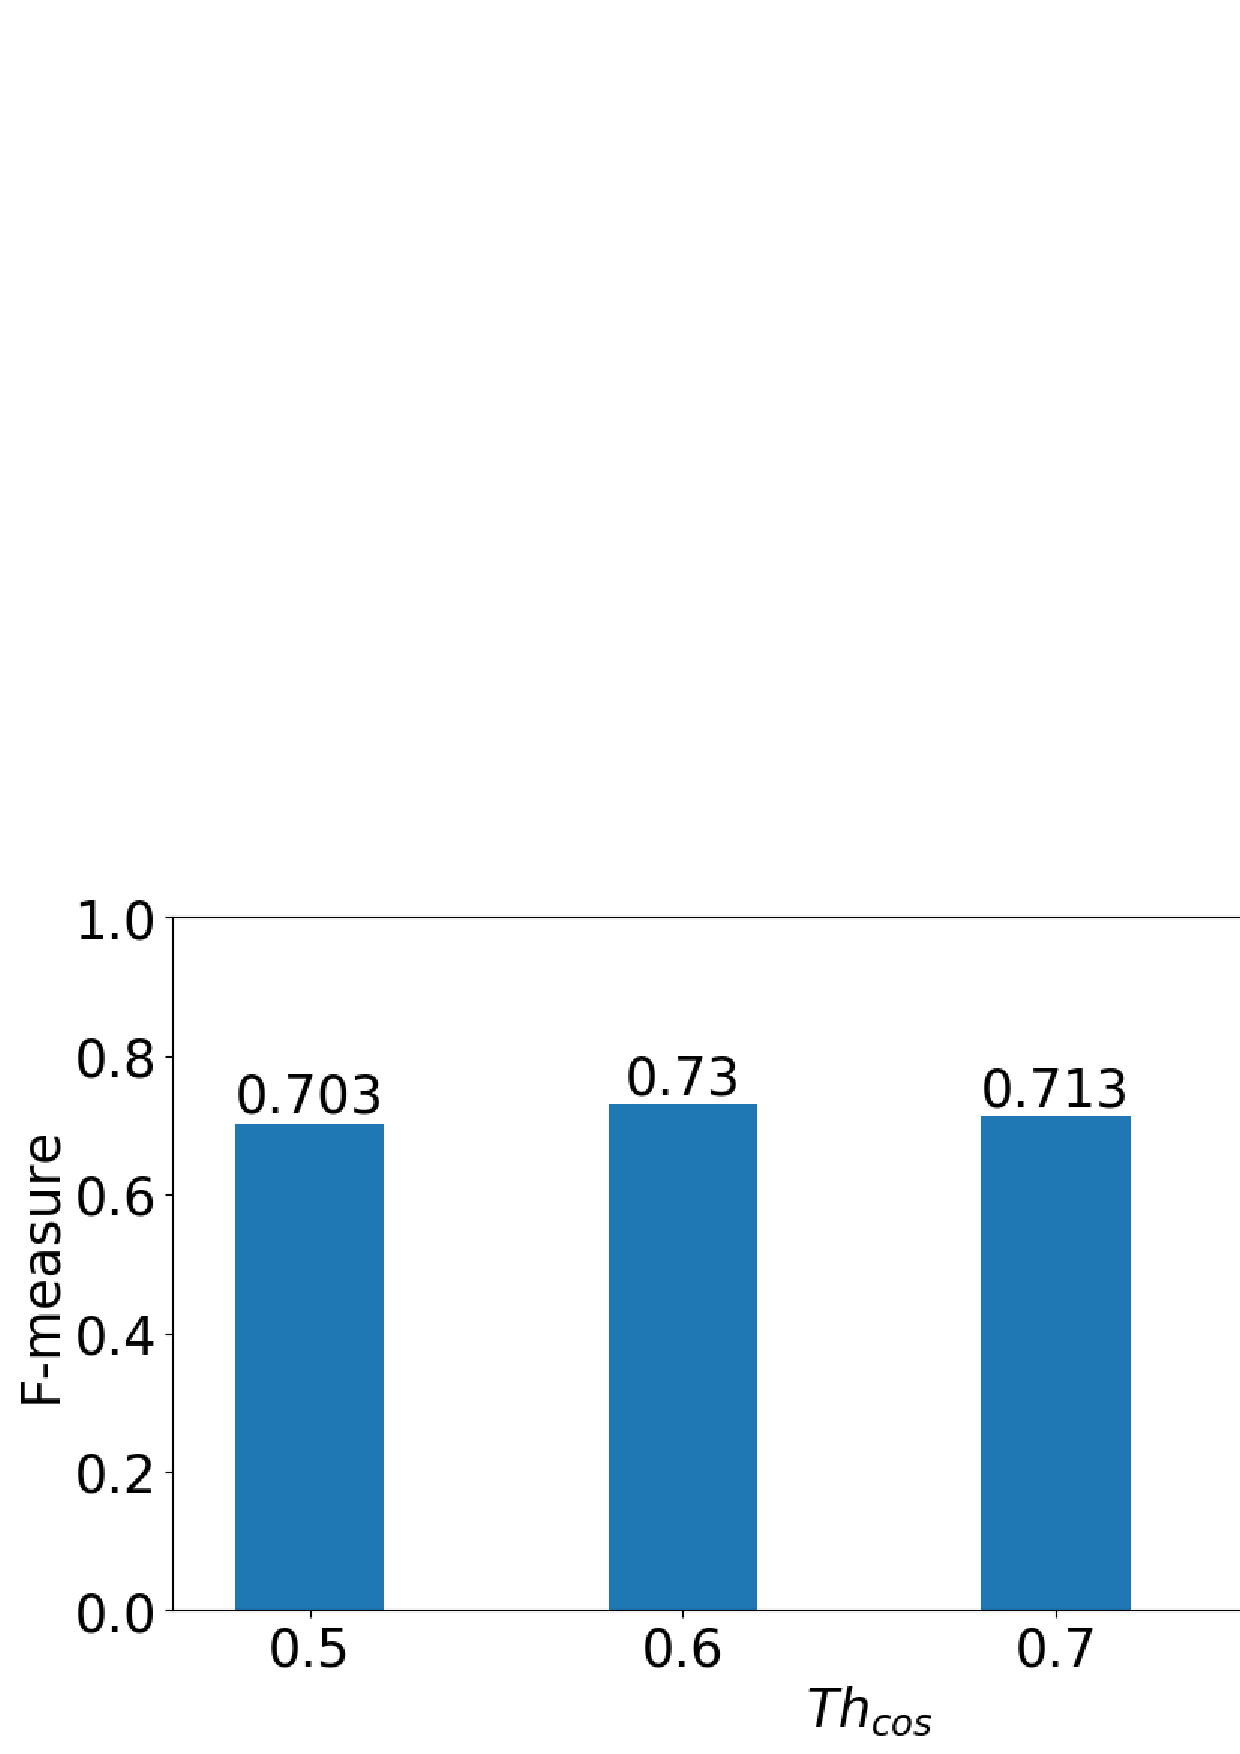
\includegraphics[keepaspectratio, scale=0.25]
                          {./figure/prob2_f.eps} \label{prob2_fmeasure}}
      \end{minipage}

      \begin{minipage}{0.06\hsize}
        \hspace{0.5mm}
      \end{minipage}
 
    \end{tabular}
\caption{手法2によるニュースアンカーの発話検出精度 \label{fig:result_anchor_prob2}}
\end{figure} 

\begin{table}[H]
  \begin{center}
    \caption{手法2による各ニュース番組音声のニュースアンカーの発話検出精度($Th_{cos}=0.6$) }
    \begin{tabular}{|c||c|c|c|c|} \hline
データID & Recall & Precision & F-meature & 作成したクラスタ数\\ \hline
ニュース1 & 0.958 & 0.617 & 0.751 & 1 \\ \hline
ニュース2 & 0.788 & 0.512 & 0.621 & 2 \\ \hline
ニュース3 & 0.695 & 0.823 & 0.754 & 2 \\ \hline
ニュース4 & 0.683 & 0.732 & 0.707 & 2 \\ \hline
ニュース5 & 0.679 & 0.960 & 0.796 & 2 \\ \hline
計 & 0.737 & 0.722 & 0.730 &  \\ \hline
    \end{tabular}
  \end{center}
\end{table}

%手法3の図
\begin{figure}[H]
  \centering
    \begin{tabular}{c}
 
%----- recall -----
 
      \begin{minipage}{0.40\hsize}
        \centering
          \subfigure[Recall]{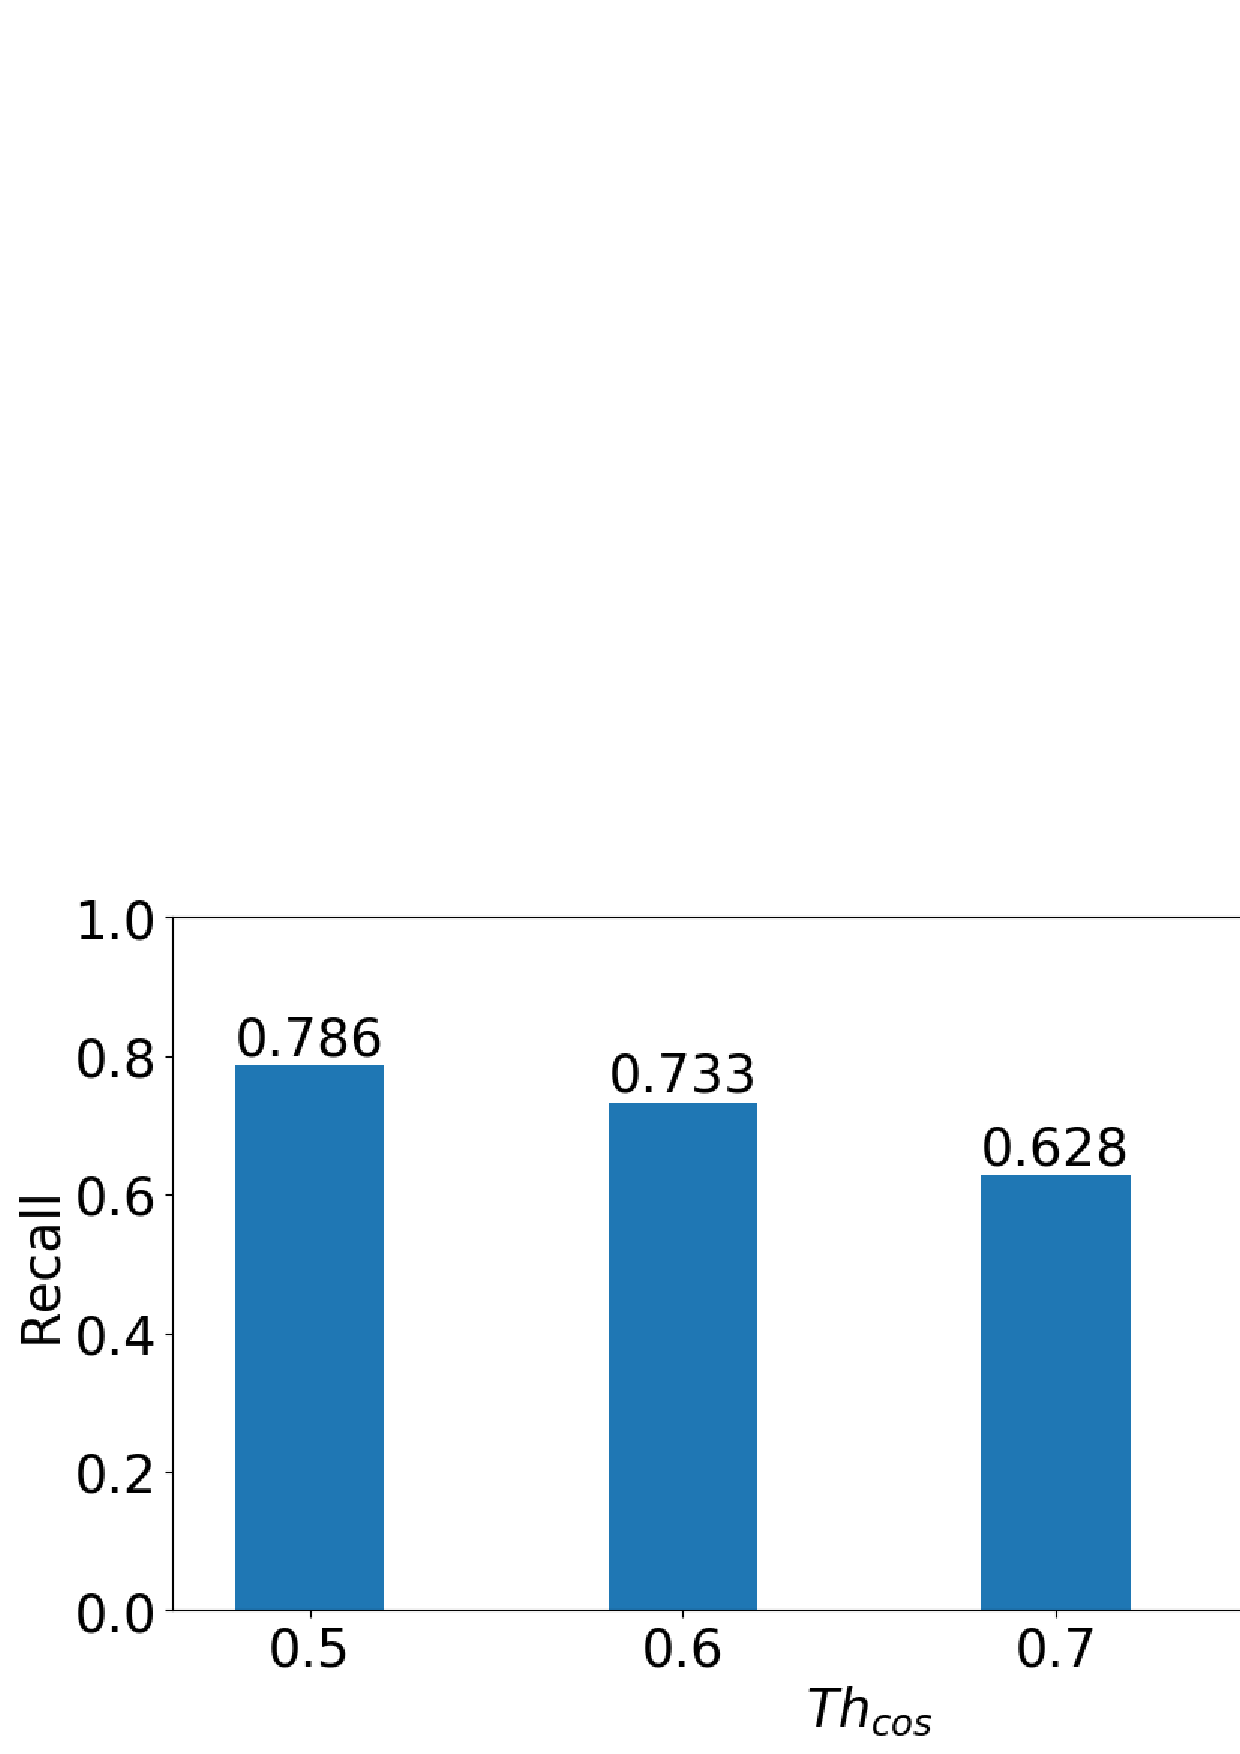
\includegraphics[keepaspectratio, scale=0.25]
                          {./figure/prob3_11_r.eps}}
      \end{minipage}

      \begin{minipage}{0.06\hsize}
        \hspace{0.5mm}
      \end{minipage}
 
%----- precision -----
 
      \begin{minipage}{0.40\hsize}
        \centering
          \subfigure[Precision]{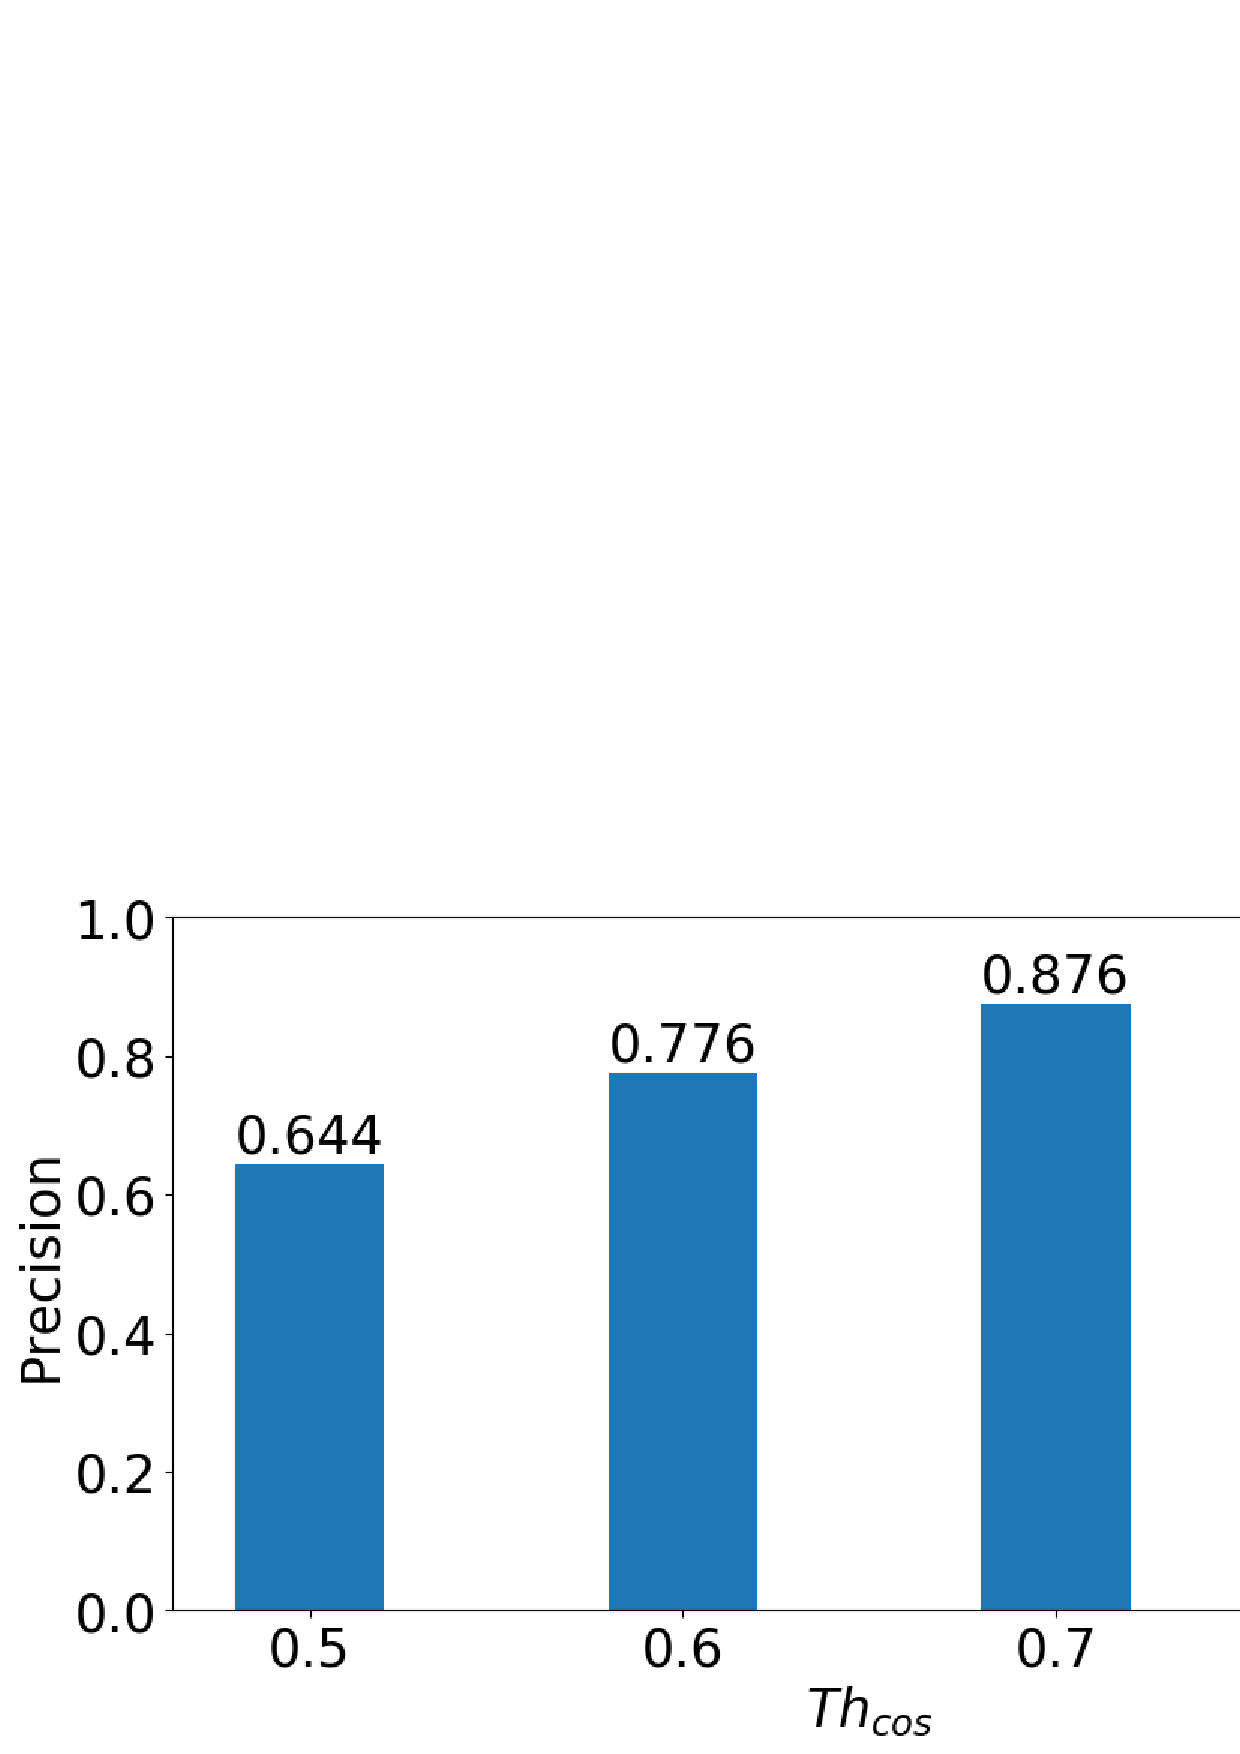
\includegraphics[keepaspectratio, scale=0.25]
                          {./figure/prob3_11_p.eps}}
      \end{minipage} \\

      \begin{minipage}{0.06\hsize}
        \vspace{5mm}
      \end{minipage} \\
 
 
%----- fmeasure -----
 
      \begin{minipage}{0.40\hsize}
        \centering
          \subfigure[F-measure]{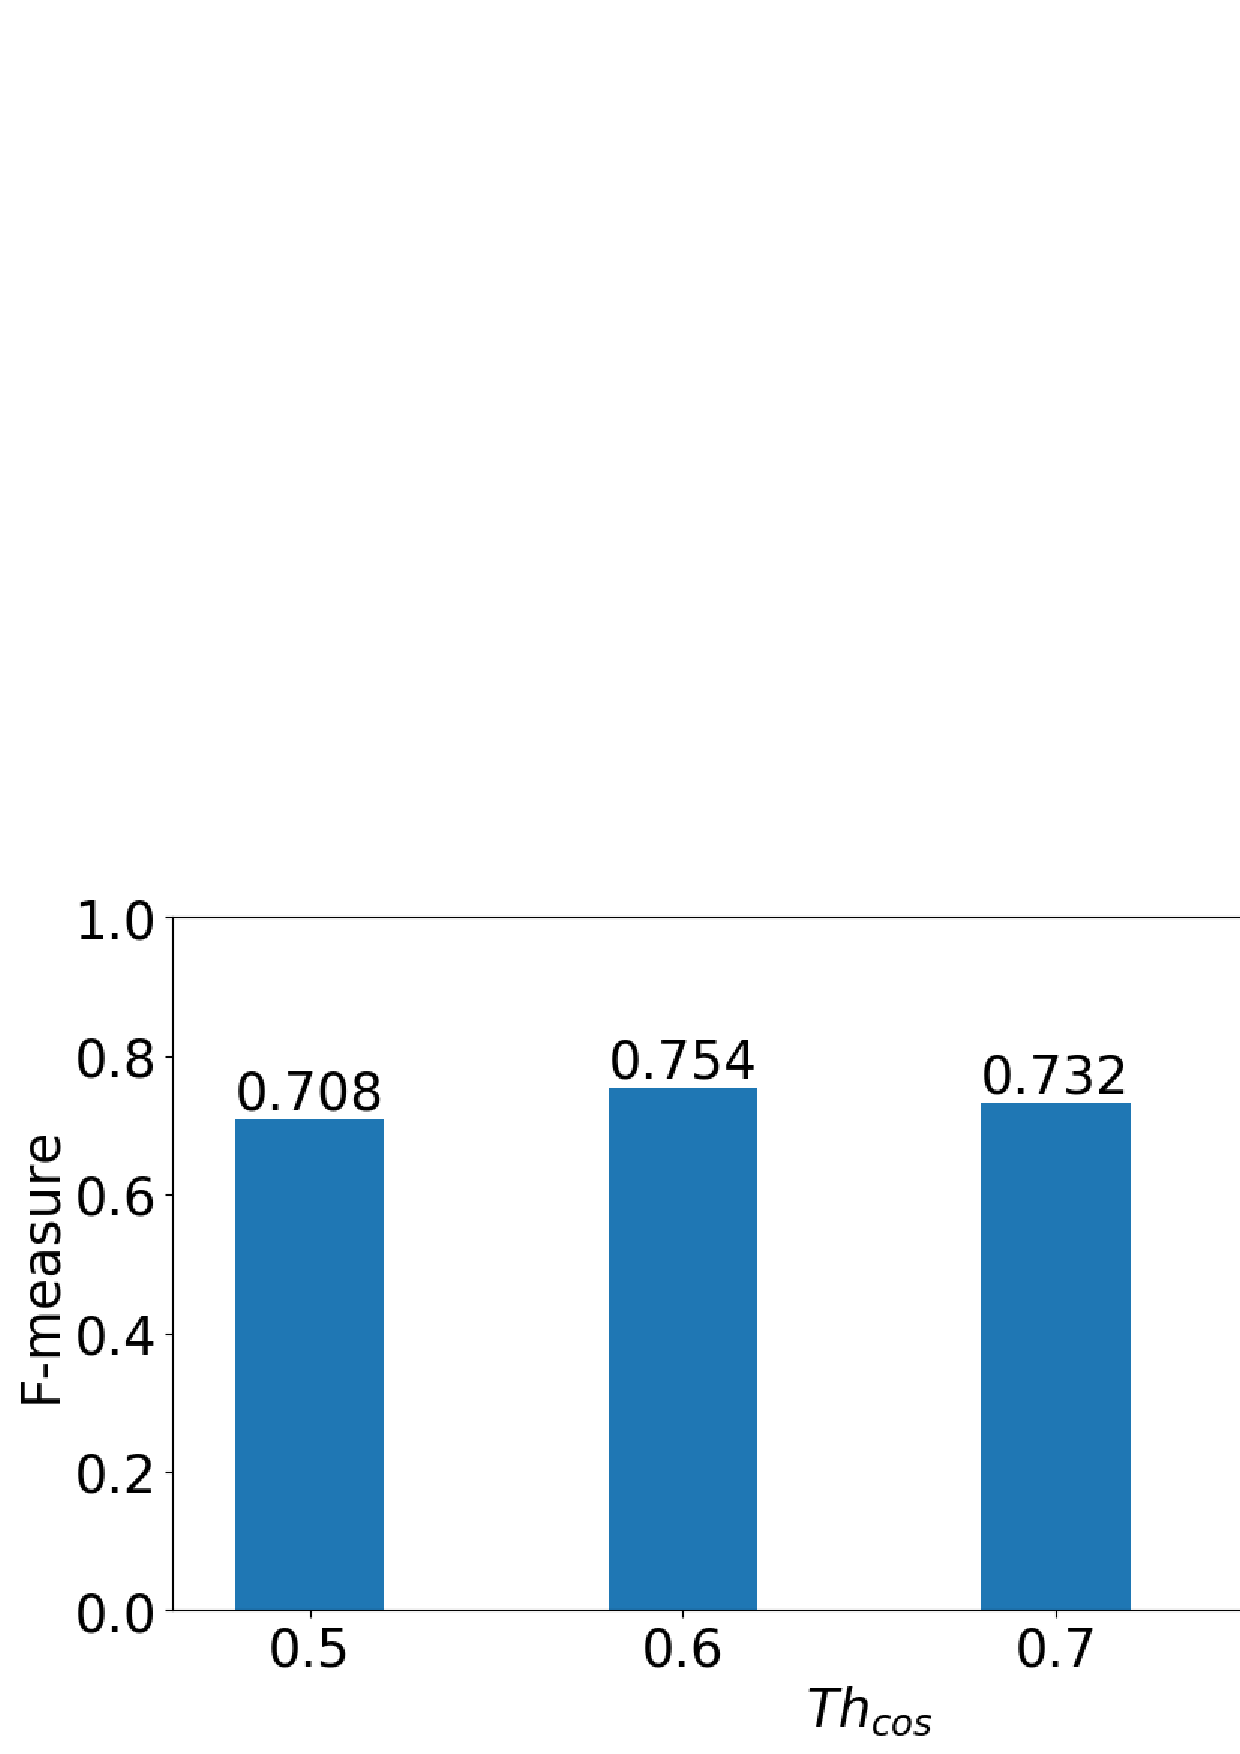
\includegraphics[keepaspectratio, scale=0.25]
                          {./figure/prob3_11_f.eps} \label{prob3_fmeasure}}
      \end{minipage}

      \begin{minipage}{0.06\hsize}
        \hspace{0.5mm}
      \end{minipage}
 
%----- acc time -----
\begin{comment}
      \begin{minipage}{0.40\hsize}
        \centering
          \subfigure[$Acc_{time}$]{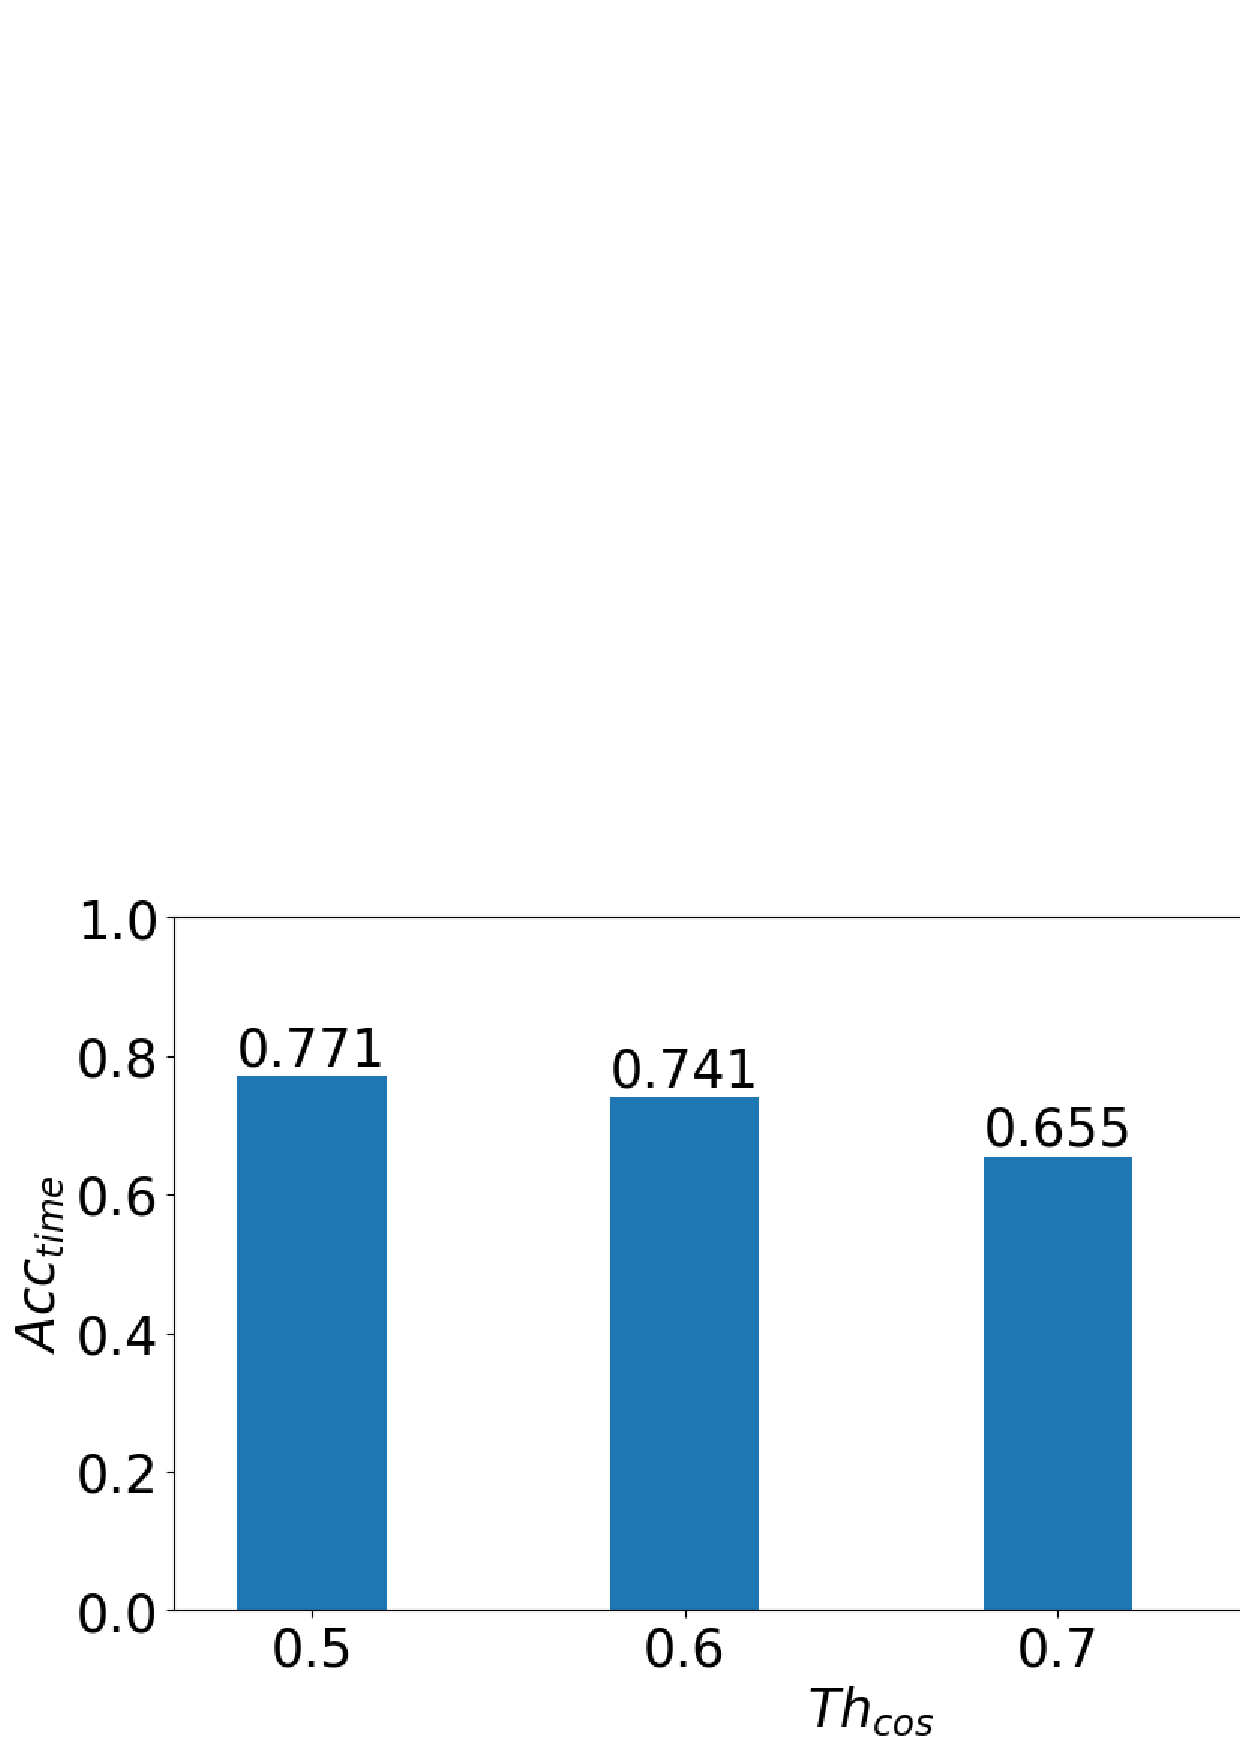
\includegraphics[keepaspectratio, scale=0.25]
                          {./figure/prob3_11_acc.eps}}
      \end{minipage}
\end{comment}
    \end{tabular}
\caption{手法3によるアンカーの発話区間検出精度 ($Th_{time}=1.1$) \label{fig:result_anchor_prob3}}
\end{figure} 


\begin{table}[H]
  \begin{center}
    \caption{手法3による各ニュース番組音声のニュースアンカーの発話検出精度($Th_{cos}=0.6,Th_{time}=1.1$) \label{table:prob3_eachnews}}
    \begin{tabular}{|c||c|c|c|c|} \hline
データID & Recall & Precision & F-meature & 作成したクラスタ数\\ \hline
ニュース1 & 0.958 & 0.702 & 0.810 & 1 \\ \hline
ニュース2 & 0.758 & 0.590 & 0.663 & 2 \\ \hline
ニュース3 & 0.725 & 0.846 & 0.781 & 2 \\ \hline
ニュース4 & 0.646 & 0.755 & 0.696 & 2 \\ \hline
ニュース5 & 0.683 & 0.973 & 0.802 & 2 \\ \hline
計 & 0.733 & 0.776 & 0.754 &  \\ \hline
    \end{tabular}
  \end{center}
\end{table}

実験の結果、Baseline2を各手法を比較したとき、ニュースアンカーの検出精度の指標であるF-measureが手法1では6.5\%(図\ref{prob1_fmeasure})、手法2では2.3\%(図\ref{prob2_fmeasure})、手法3では4.7\%(図\ref{prob3_fmeasure})の向上が確認された。また、Baselineと提案手法の全てにおいてニュース2の検出精度であるPrecisionが最も低い。\par
いずれの手法においても$Th_{cos}$が小さい時にはRecallが高く、大きい時にはPrecisionが高くなる傾向が確認された。また、$Acc_{time}$は$Th_{cos}$が大きくなると低くなる傾向にある。また、Baseline1を除く全ての手法でニュースアンカーの人数と検出したニュースアンカーの人数が同じであった。\par